%===============================================================================
% Dissertação de Mestrado - Marcelo B. da Cruz
% Migrado do paper IEEEtran (sbaconf) para o template CoppeTeX (PESC/COPPE/UFRJ)
%
% Pré-requisitos no diretório:
%   - coppe.cls
%   - coppe-unsrt.bst (ou coppe-plain.bst)
%   - coppe.ist
%   - latexmkrc (opcional, para gerar listas de símbolos/abreviaturas)
%   - bibliografy.bib
%   - Figuras em figuras/ referenciadas no texto
%===============================================================================
% Use a opção [numbers] se preferir citações no estilo numérico [1].
% Sem [numbers], natbib usa formato autor-ano (Pereira & Pinto, 1991).
\documentclass[msc]{coppe}

\usepackage{booktabs}              % tabelas mais elegantes
\usepackage{rotating}              % sidewaystable, se necessário
\usepackage{longtable}             % tabelas longas
\usepackage[most]{tcolorbox}       % caixas de texto
\usepackage{amsmath,amssymb}
\usepackage{graphicx}
\graphicspath{{figuras/}}
\usepackage{xcolor}                % preserva os ToDo's em vermelho do paper original
\usepackage{url}
\usepackage{hyperref}
\usepackage{listings}              % opcional, para trechos de código
\usepackage{float}                 % opção [H] para fixar posição de figuras
\usepackage{placeins}              % \FloatBarrier para conter floats em seções

\makelosymbols
\makeloabbreviations

\begin{document}

  \title{Investigando Problemas de Escalabilidade de E/S no Algoritmo SDDP em Ambientes HPC}
  \foreigntitle{Investigating I/O Scalability Issues in the SDDP Algorithm on HPC Environments}
  \author{Marcelo}{Barros da Cruz}
  \advisor{Prof.}{Nome do Orientador}{Sobrenome}{D.Sc.}
  % Acrescente \advisor adicionais se houver coorientação:
  % \advisor{Prof.}{Nome do Coorientador}{Sobrenome}{D.Sc.}
  \examiner{Prof.}{Nome do Primeiro Examinador Sobrenome}{D.Sc.}
  \examiner{Prof.}{Nome do Segundo Examinador Sobrenome}{D.Sc.}
  \examiner{Prof.}{Nome do Terceiro Examinador Sobrenome}{D.Sc.}
  \department{PESC}
  \date{04}{2026}

  \keyword{MPI-IO}
  \keyword{Lustre}
  \keyword{SDDP}
  \keyword{Computação de Alto Desempenho}
  \keyword{Escalabilidade de E/S}

  \maketitle

  \frontmatter

  \dedication{Dedico esta dissertação a \textbf{[a definir]}.}

  \chapter*{Agradecimentos}
  \textcolor{red}{\textbf{ToDp: redigir agradecimentos finais.}}
  Coloque aqui seus agradecimentos.

  \begin{abstract}
  A escalabilidade eficiente de E/S continua sendo um desafio crítico em
  aplicações paralelas de dados massivos, especialmente em sistemas de alto
  desempenho que lidam com grandes volumes de dados. Embora avanços como o uso
  de MPI-IO e sistemas de arquivos paralelos como o Lustre tenham contribuído
  significativamente, muitas aplicações ainda enfrentam gargalos que
  comprometem a performance. Esse problema é particularmente evidente em
  modelos de otimização utilizados no setor energético, como o SDDP, que
  demandam acesso frequente e distribuído a grandes conjuntos de dados. A
  eficiência da E/S torna-se, assim, um fator decisivo para a viabilidade e o
  desempenho de simulações complexas em ambientes paralelos. Esta dissertação
  investiga os gargalos de E/S do algoritmo SDDP e propõe uma arquitetura MPI-IO baseada em MPI-IO sobre Lustre, avaliada empiricamente nos
  ambientes AWS (FSx for Lustre) e Santos Dumont (LNCC).
  \end{abstract}

  \begin{foreignabstract}
  Efficient I/O scalability remains a major challenge for parallel
  applications handling massive data volumes, particularly in
  high-performance computing environments. Although advances such as MPI-IO
  and parallel file systems like Lustre have significantly improved
  performance, many applications still face I/O bottlenecks that hinder
  scalability. This issue is particularly critical in energy sector
  optimization models, such as Stochastic Dual Dynamic Programming (SDDP),
  which require frequent and distributed access to large datasets. Therefore,
  optimizing I/O operations becomes essential to ensure the feasibility and
  efficiency of complex simulations in parallel computing systems. This
  dissertation investigates the I/O bottlenecks of the SDDP algorithm and
  proposes an MPI-IO-based architecture over Lustre,
  empirically evaluated on AWS (FSx for Lustre) and on the Santos Dumont
  supercomputer (LNCC).
  \end{foreignabstract}

  \tableofcontents
  \listoffigures
  \listoftables
  \printlosymbols
  \printloabbreviations

  \mainmatter

%===============================================================================

%===============================================================================
\chapter{Introdução}
\label{cap:introducao}

\abbrev{HPC}{High-Performance Computing}
\abbrev{MPI}{Message Passing Interface}
\abbrev{E/S}{Entrada/Saída}
\abbrev{SDDP}{Stochastic Dual Dynamic Programming}

O aumento da complexidade e do volume de dados em aplicações científicas e
de engenharia tem tornado a computação paralela uma ferramenta indispensável
para atender às demandas de desempenho~\cite{Kang:20}. Entretanto,
operações de entrada e saída (E/S) continuam sendo um dos principais gargalos
em ambientes de alto desempenho (HPC), particularmente em aplicações que
processam dados massivos~\cite{Luu:15, Xie:20}. Nesse contexto, o uso de
bibliotecas como o MPI-IO, combinadas com sistemas de arquivos paralelos como
o Lustre, tornou-se uma abordagem fundamental para lidar com a escalabilidade
e a eficiência no acesso aos dados~\cite{mpi50Cite, LustreManual}.

Paralelamente, a crescente inserção de fontes renováveis na matriz
energética, como solar e eólica, tem introduzido novas dificuldades na
formulação e resolução de problemas de otimização associados à operação dos
sistemas elétricos. A variabilidade e incerteza dessas fontes requerem
modelos computacionais mais complexos e dependentes de grandes volumes de
dados, cuja execução eficiente depende tanto do paralelismo computacional
quanto de soluções eficazes de E/S~\cite{Ajc:10, Ssr:19}.

\textcolor{red}{\textbf{ToDp: precisamos expandir esse parágrafo, explicar o
que implica essa mudança de paradigma na simulação tanto para o uso de
recursos computacionais como para o uso dos resultados pelos usuários do
SDDP.}}

Assim como outras aplicações baseadas em tarefas independentes, o modelo
SDDP (\textit{Stochastic Dual Dynamic Programming}) é amplamente utilizado
para planejamento e despacho hidrotérmico em diversos países. À medida que
os modelos se tornam mais detalhados, em resolução horária, e a quantidade
de cenários aumenta, a execução do SDDP passa a demandar não apenas alto
poder computacional, mas também operações intensivas de E/S~\cite{MvLm:91}.

Nesse contexto, esta dissertação investiga o desempenho do MPI-IO sobre
sistemas de arquivos paralelos como o Lustre nessa classe de aplicações,
com foco no comportamento da E/S em ambientes HPC.

Esta dissertação concentra-se na fase de simulação final do SDDP ---
etapa executada após a convergência da política de operação, na qual um
conjunto fixo de cortes de Benders é avaliado em larga escala sobre
múltiplos cenários para produzir os resultados operacionais entregues ao
planejamento. As escolhas algorítmicas relacionadas à construção da
política (fase iterativa de geração de cortes) estão fora do escopo
deste trabalho.

\textcolor{red}{\textbf{ToDp: Apresentar organização da dissertação ao final
da introdução (capítulos 2--5).}}



%===============================================================================
\chapter{Fundamentação Teórica}
\label{cap:fundamentacao}

\abbrev{MPI-IO}{MPI Input/Output}
\abbrev{OST}{Object Storage Target}
\abbrev{MDS}{Metadata Server}
\abbrev{MDT}{Metadata Target}
\abbrev{OSS}{Object Storage Server}
\abbrev{RDMA}{Remote Direct Memory Access}
\abbrev{AWS}{Amazon Web Services}
\abbrev{FSx}{Amazon FSx for Lustre}
\abbrev{EFA}{Elastic Fabric Adapter}
\abbrev{ONS}{Operador Nacional do Sistema Elétrico}
\abbrev{PMO}{Programa Mensal da Operação}
\abbrev{SIN}{Sistema Interligado Nacional}
\abbrev{LNCC}{Laboratório Nacional de Computação Científica}
\abbrev{SINAPAD}{Sistema Nacional de Processamento de Alto Desempenho}

\section{MPI e protocolos de comunicação}
O \textit{Message Passing Interface} (MPI) é o padrão para programação
paralela baseada em troca de dados entre processos, sendo amplamente utilizado em
\textit{clusters} e supercomputadores. Um aspecto essencial da sua
implementação são os protocolos de comunicação: o \textit{eager}, que envia
pequenos blocos de dados de forma imediata, sem necessidade de confirmação do
receptor, favorecendo baixa latência; e o \textit{rendezvous}, que aguarda o
\textit{handshake} do receptor antes de transmitir blocos de dados maiores,
reduzindo \textit{overhead} de memória e aumentando a previsibilidade do
desempenho em cargas intensivas~\cite{mpiCite}. A escolha entre os
protocolos depende fortemente do tamanho do bloco de dados e da disponibilidade de
\textit{buffers}: enquanto o \textit{eager} utiliza \textit{buffers}
internos para armazenar temporariamente dados até que o receptor os
processe, o \textit{rendezvous} elimina essa necessidade para blocos de dados
grandes, evitando consumo excessivo de memória e garantindo maior
estabilidade em aplicações de larga escala~\cite{Wea:99,Rrw:05}.

\section{MPI-IO e operações paralelas de arquivos}
O MPI também estende suas funcionalidades à entrada e saída de dados por
meio da especificação MPI-IO~\cite{mpiioCite}, que define uma API
padronizada para operações paralelas de arquivos. Essa interface possibilita
que múltiplos processos acessem simultaneamente grandes volumes de dados,
permitindo otimizações como \textit{collective I/O}, técnicas de agregação e
\textit{data sieving}, que reduzem o número de operações pequenas e melhoram
a eficiência do uso do sistema de arquivos. Entre as chamadas mais
utilizadas, destacam-se \texttt{MPI\_File\_write\_at}, que realiza uma
escrita independente em um deslocamento específico do arquivo, permitindo
controle preciso sobre onde os dados serão gravados, e
\texttt{MPI\_File\_write\_all}, que executa uma operação coletiva em que
todos os processos participantes escrevem de forma coordenada. Enquanto a
primeira é adequada para acessos irregulares ou não sincronizados, a segunda
explora a comunicação coletiva para reduzir \textit{overhead} de metadados e
alinhar requisições, sendo mais eficiente em ambientes com sistemas de
arquivos distribuídos como o Lustre.

\section{Sistema de arquivos paralelo Lustre}
Projetado especificamente para cargas massivas de HPC, ele distribui os
dados em \textit{Object Storage Targets} (OSTs) e os metadados em
\textit{Metadata Servers} (MDS), permitindo acesso paralelo e balanceado a
múltiplos clientes. Além disso, o Lustre utiliza a técnica de
\textit{striping}, na qual um arquivo é dividido em blocos
(\textit{chunks} ou \textit{stripes}) distribuídos entre diferentes OSTs.
O tamanho do \textit{stripe} e o número de OSTs utilizados podem ser
configurados de acordo com o padrão de acesso da aplicação, influenciando
diretamente no \textit{throughput} e na escalabilidade: \textit{stripes}
maiores tendem a favorecer grandes operações sequenciais, enquanto
\textit{stripes} menores podem beneficiar acessos concorrentes e
distribuídos~\cite{Pjb:02}. Graças a essa flexibilidade e alto desempenho,
o Lustre tornou-se amplamente adotado em supercomputadores listados no
TOP500, constituindo um elemento-chave para aplicações científicas e
industriais que exigem desempenho extremo em E/S.

\section{Adaptadores de rede em HPC: Ethernet e InfiniBand}
Os adaptadores de rede são componentes críticos para o desempenho em
sistemas de computação de alto desempenho, sendo a Ethernet e o InfiniBand
as tecnologias mais utilizadas. A Ethernet, tradicionalmente projetada para
redes locais corporativas, evoluiu para padrões de alta velocidade, como
40/100/400~Gbps, oferecendo elevada taxa de transferência
(\textit{bandwidth}), embora apresente latências relativamente maiores,
frequentemente na ordem de dezenas de microssegundos. Já o InfiniBand foi
desenvolvido especificamente para ambientes de HPC, combinando altas
larguras de banda --- que podem ultrapassar 400~Gbps em implementações
modernas --- com latências extremamente baixas, tipicamente abaixo de
2~$\mu$s, graças a recursos como comunicação RDMA (\textit{Remote Direct
Memory Access}). Essa diferença torna o InfiniBand preferido em
supercomputadores e \textit{clusters} científicos, onde a baixa latência na
troca de dados entre processos é tão relevante quanto a banda disponível, enquanto a
Ethernet, pelo menor custo e ampla compatibilidade, mantém espaço em
sistemas híbridos e \textit{datacenters}~\cite{Fds:03,RlGmmts:05}.

\section{Computação em nuvem para HPC: AWS}
A Amazon Web Services (AWS) tem se consolidado como uma das principais
plataformas de computação em nuvem para aplicações de \textit{High
Performance Computing} (HPC), oferecendo recursos sob demanda que permitem
a execução de cargas de trabalho intensivas em computação e E/S. Entre os
serviços disponíveis, destacam-se as instâncias otimizadas para HPC, como
as famílias C, H e P, que fornecem alto poder de processamento aliado a
interconexões de baixa latência por meio do \textit{Elastic Fabric Adapter}
(EFA), permitindo a utilização de bibliotecas como MPI em escala. Para
atender aplicações intensivas em dados, a AWS integra sistemas de
armazenamento de alto desempenho, como o Amazon FSx for Lustre, que
viabiliza acesso paralelo e em larga escala, semelhante a sistemas de
arquivos utilizados em supercomputadores tradicionais. Essa combinação de
infraestrutura elástica, rede de alto desempenho e suporte a ferramentas
amplamente usadas em HPC torna a nuvem da AWS uma alternativa competitiva
frente a \textit{clusters} locais, especialmente em cenários que demandam
escalabilidade e flexibilidade~\cite{Krlkssj:10,Hmns:20}.

\section{O Programa Mensal da Operação (PMO)}
No setor elétrico brasileiro, o Programa Mensal da Operação (PMO) é um
documento técnico elaborado pelo Operador Nacional do Sistema Elétrico
(ONS) que estabelece as diretrizes de curto prazo para a operação do
Sistema Interligado Nacional (SIN). O PMO contempla projeções de carga,
disponibilidade de geração, restrições de transmissão e condições
hidrológicas, servindo como referência para a programação da operação
hidrotérmica de forma a garantir o equilíbrio entre oferta e demanda de
energia elétrica. Além disso, define metas de despacho de usinas
hidrelétricas e termelétricas, contribuindo para a segurança energética e
para a otimização do uso dos recursos disponíveis. Por sua relevância, o
PMO orienta não apenas as decisões operativas do ONS, mas também agentes
do setor, incluindo geradores, comercializadores e distribuidores, sendo
um instrumento fundamental para a gestão integrada e eficiente do
SIN~\cite{ons:23}.

\section{Algoritmo SDDP}
O algoritmo SDDP (\textit{Stochastic Dual Dynamic Programming}),
proposto por~\cite{MvLm:91}, decompõe o problema de planejamento
hidrotérmico em uma malha bidimensional de subproblemas
determinísticos: cada subproblema é indexado por um par
$(\text{estágio}, \text{cenário})$, em que os estágios representam
períodos discretos da operação --- meses, no caso da operação
programada do SIN --- e os cenários representam realizações
estocásticas das variáveis relevantes, principalmente afluências aos
reservatórios. A solução do problema é construída de forma iterativa,
combinando simulações ao longo dos cenários e refinamentos da política
de operação até a convergência.

A Figura~\ref{fig:SDDP_cenarios_estagios} esquematiza a estrutura de
subproblemas resolvida pelo SDDP nas configurações adotadas nos
experimentos desta dissertação: três estágios mensais e $1\,536$
cenários, totalizando $4\,608$ subproblemas. Os cenários são, por
construção, independentes entre si --- cada cenário corresponde a uma
realização estocástica distinta, sem compartilhamento de estado com os
demais. Essa propriedade caracteriza o SDDP como uma aplicação do tipo
\textit{bag-of-tasks}~\cite{Cirne:2003}: um conjunto de tarefas
mutuamente independentes que podem ser distribuídas entre processadores
sem coordenação durante a execução. Os cenários são particionados entre
os \textit{ranks} MPI e resolvidos em paralelo, de modo que o tempo
total da fase de simulação fica limitado pelo cenário mais lento e não
pela soma sequencial de todos. A natureza \textit{bag-of-tasks} do SDDP
é o que torna o algoritmo escalável em sistemas HPC; é também o que
desloca o gargalo da computação para a persistência dos resultados, à
medida que o número de cenários cresce.

Após a resolução, os resultados de cada subproblema --- variáveis
primais, multiplicadores duais e custos --- precisam ser persistidos em
disco, pois alimentam etapas subsequentes do próprio algoritmo e
análises estatísticas posteriores.

A granularidade temporal adotada para os resultados de cada estágio tem
impacto direto sobre o volume de dados produzido por iteração. A
abordagem tradicional do SDDP agrega a operação dentro de cada estágio
em poucos blocos representativos de carga (\textit{patamares}: pesado,
médio e leve), reduzindo cada estágio a um pequeno número de pontos
operativos por cenário. A operação programada moderna, entretanto,
especialmente com a crescente penetração de fontes intermitentes como
solar e eólica, requer resolução horária para capturar adequadamente
horários de ponta, vales e rampas associadas à variabilidade dessas
fontes. Esta dissertação foca exatamente no regime de resultados
horários, em que cada estágio de um cenário gera dados proporcionais ao
número de horas simuladas --- ordem de magnitude maior que o caso
tradicional por blocos. É nesse regime que o gargalo de E/S se torna
efetivamente dominante: o volume agregado escrito por iteração cresce
linearmente com o número de cenários, com o número de estágios e com a
granularidade temporal interna de cada estágio, e a estratégia de
implementação dessas escritas determina diretamente a escalabilidade da
aplicação em ambientes HPC.

\begin{figure}[H]
  \centering
  
\includegraphics[width=\textwidth]{SDDP_cenarios_estagios.png}
  \caption{Estrutura de cenários e estágios do SDDP nos experimentos
  desta dissertação. Cada célula corresponde a um subproblema
  $(\text{estágio}, \text{cenário})$. Os cenários são mutuamente
  independentes e podem ser distribuídos entre \textit{ranks} MPI,
  caracterizando uma aplicação \textit{bag-of-tasks}.}
  \label{fig:SDDP_cenarios_estagios}
\end{figure}

\subsection{Arquitetura atual de E/S do SDDP com um único processo escritor}
\label{sec:arq_atual}
Na arquitetura atual do SDDP, apenas um \textit{rank} MPI (o
\textit{rank}~1) é designado para realizar todas as operações de E/S do
sistema. Cada nó de computação, após resolver sua respectiva tarefa, envia
os resultados por meio de um \textit{buffer} de dados utilizando a função
\texttt{MPI\_Send}. Esse \textit{buffer} é então recebido pelo processo
escritor através de uma chamada \texttt{MPI\_Recv} e, posteriormente, os
dados são gravados em um sistema de arquivos distribuído. A
Figura~\ref{fig:SDDP_architecture} ilustra o funcionamento dessa
arquitetura.

\begin{figure}[H]
  \centering
  
\includegraphics[width=0.7\textwidth]{SDDP_architecture.png}
  \caption{Algoritmo SDDP com processo escritor.}
  \label{fig:SDDP_architecture}
\end{figure}

Independentemente do número de nós computacionais utilizados, apenas um
processo é responsável pelas operações de E/S. Cada nó utiliza sua banda
efetiva para enviar os \textit{buffers} de dados, enquanto o processo
escritor utiliza sua banda para recebê-los. A primeira hipótese para as
limitações de escalabilidade nessa arquitetura está relacionada ao
adaptador de rede do servidor que executa o processo mestre.

Adicionalmente, o \textit{rank}~0 é responsável pelo gerenciamento e
controle da aplicação, como a distribuição de tarefas para os demais
\textit{ranks} e o envio/recebimento das configurações do sistema. Essas
atividades também utilizam o mesmo adaptador de rede empregado na
recepção dos \textit{buffers} de dados. Outra hipótese é que o processo
escritor opera continuamente em um fluxo sequencial de recepção e escrita
dos dados, o que pode representar um gargalo adicional, sobretudo em
sistemas com alto volume de dados. Por fim, se houver atrasos na recepção
ou na gravação dos \textit{buffers} de dados por parte do processo mestre,
os nós computacionais podem ser obrigados a aguardar, gerando sobrecarga
no envio dos \textit{buffers} e aumentando o custo computacional da
execução paralela.



%===============================================================================
\chapter{Paralelização dos Mecanismos de E/S do SDDP}
\label{cap:proposta}

Este capítulo apresenta a proposta de paralelização dos mecanismos de
entrada e saída (E/S) do SDDP. A solução substitui o modelo atual,
por uma organização baseada em MPI-IO sobre
o sistema de arquivos Lustre. Nessa abordagem, cada \textit{rank} grava
diretamente seus próprios resultados em regiões independentes do espaço de
saída, evitando a concentração das operações de E/S em um único processo.

O ponto central da proposta é explorar, simultaneamente, o paralelismo da
aplicação MPI e o paralelismo do sistema de arquivos. Como os resultados
produzidos por diferentes \textit{ranks} são independentes, suas escritas
podem ser posicionadas previamente e executadas em paralelo. No Lustre, os
arquivos são distribuídos em \textit{stripes} entre diferentes
\textit{Object Storage Targets} (OSTs); assim, múltiplas escritas
independentes podem ser atendidas por OSTs distintos, aumentando a largura
de banda agregada e reduzindo a contenção observada no modelo com escritor
centralizado.

Dessa forma, a proposta visa reduzir dois gargalos da arquitetura original. O
primeiro é o gargalo de comunicação, pois os dados deixam de ser enviados
ao processo escritor antes de serem persistidos. O segundo é o gargalo de
armazenamento, pois a escrita passa a ser distribuída entre os recursos do
sistema de arquivos paralelo, em vez de ser serializada por um único
\textit{rank}. A Figura~\ref{fig:SDDP_architecture2} sintetiza essa nova
organização.

\section{Uso de MPI-IO com Lustre para escalabilidade de E/S}
Como hipótese para mitigar essas limitações, propõe-se a substituição do modelo atual de E/S por uma abordagem MPI-IO, baseada na interface
MPI-IO em conjunto com o sistema de arquivos distribuído Lustre.

A interface MPI-IO, parte do padrão MPI-2, fornece mecanismos para a
realização de operações de E/S por múltiplos processos MPI sobre arquivos
compartilhados. Diferentemente do modelo tradicional de comunicação ponto a
ponto (\texttt{MPI\_Send}/\texttt{MPI\_Recv}), o MPI-IO permite que cada
processo realize operações diretas de escrita em arquivos, sem a
necessidade de coordenação com um processo único de escrita~\cite{Rwe:99}. Essa flexibilidade
possibilita que os próprios processos responsáveis pela computação escrevam
seus resultados diretamente em disco, utilizando \textit{offsets} distintos
e evitando conflitos de acesso. Isso é particularmente relevante em
aplicações como o SDDP, em que os dados produzidos por cada \textit{rank}
são independentes e podem ser gravados em posições previamente determinadas
de um arquivo compartilhado, ou mesmo em arquivos separados.

Aliado ao MPI-IO, propõe-se o uso do sistema de arquivos Lustre, amplamente
adotado em ambientes de computação de alto desempenho (HPC). O Lustre foi
projetado para oferecer alto rendimento e paralelismo no acesso a arquivos,
distribuindo os dados entre múltiplos servidores de armazenamento (OSTs ---
\textit{Object Storage Targets})~\cite{Pjb:02}. Essa característica torna o
Lustre particularmente eficiente em cenários onde múltiplos nós executam
operações simultâneas de escrita, como se espera com a integração do
MPI-IO. A combinação das duas tecnologias permite que os \textit{ranks}
MPI realizem operações de E/S em paralelo, aproveitando ao máximo a largura
de banda disponível no sistema e reduzindo significativamente os gargalos
causados pela concentração da escrita.

Espera-se que essa nova arquitetura traga ganhos substanciais de
desempenho. Primeiramente, ao eliminar o processo escritor único, a
aplicação poderá distribuir dinamicamente a carga de E/S entre os próprios
processos computacionais, reduzindo a sobrecarga sobre o adaptador de rede
do nó mestre. Em segundo lugar, a redução da dependência de
\textit{buffers} intermediários e de sincronizações entre \textit{ranks}
minimiza a latência entre o término da computação e a persistência dos
resultados. Além disso, a utilização do paralelismo nativo do Lustre deverá
resultar em um melhor aproveitamento dos recursos de armazenamento,
tornando o sistema mais escalável à medida que aumenta o número de nós.
Por fim, essa abordagem alinha-se às boas práticas adotadas em aplicações
científicas de larga escala, promovendo maior portabilidade, eficiência e
adaptabilidade a infraestruturas HPC modernas. A
Figura~\ref{fig:SDDP_architecture2} descreve o funcionamento da proposta.

\section{Organização dos arquivos compartilhados de resultados}
\label{sec:arquivos_compartilhados_sddp}

Os resultados gerados pelo SDDP são organizados em arquivos de saída com
dimensões associadas a estágio, cenário e hora. A dimensão estágio pode
representar meses ou semanas, dependendo da base de dados utilizada, enquanto
as dimensões cenário e hora representam, respectivamente, as realizações
estocásticas simuladas e a discretização horária dos resultados. Assim, cada
registro de saída pode ser identificado por uma tupla
$(e,c,h)$, em que $e$ indica o estágio, $c$ o cenário e $h$ a hora.

Na arquitetura proposta, esses resultados podem ser gravados em arquivos
compartilhados por múltiplos processos MPI. A escrita permanece
independente: cada \textit{rank} calcula previamente a região do arquivo que
corresponde aos resultados sob sua responsabilidade e escreve diretamente
nessa posição por meio de chamadas MPI-IO com \textit{offset} explícito,
como \texttt{MPI\_File\_write\_at} ou sua variante não bloqueante. Com isso,
não é necessário encaminhar todos os blocos para um processo escritor central,
e também não é necessário sincronizar todos os processos em uma operação
coletiva de escrita.

Considerando um arquivo linearizado na ordem estágio--cenário--hora, o
\textit{offset} de um registro pode ser calculado a partir de

\begin{equation}
  \textit{offset}(e,c,h) =
  \textit{base} + (((e \times N_c + c) \times N_h + h) \times S_r),
\end{equation}

em que $N_c$ é o número de cenários, $N_h$ é o número de horas por estágio e
$S_r$ é o tamanho, em bytes, de cada registro de resultado. Essa organização
permite que cada processo escreva em uma região disjunta do arquivo. Quando
um \textit{rank} é responsável por um conjunto contíguo de cenários, horas ou
estágios, a escrita pode ser emitida como um bloco contíguo, evitando o uso de
\textit{strides} ou de \textit{file views} complexas. Essa é uma vantagem
importante para o SDDP, pois reduz a complexidade da descrição do acesso e
favorece requisições maiores ao sistema de arquivos.

A escolha por escrita independente, em vez de escrita coletiva, decorre do
padrão de execução do SDDP. Os subproblemas associados aos cenários podem
terminar em momentos diferentes, e impor uma sincronização global para gravar
resultados pode introduzir espera artificial entre processos. Além disso,
quando os resultados são produzidos em blocos pequenos, sincronizar todos os
\textit{ranks} a cada etapa de escrita pode aumentar a contenção e reduzir a
sobreposição entre computação e E/S. A escrita independente com
\textit{offsets} explícitos preserva a autonomia dos processos e permite que a
aplicação explore uma abordagem assíncrona: os blocos já produzidos podem ser
encaminhados ao sistema de arquivos enquanto outros processos continuam
avançando na computação.

No Lustre, o arquivo compartilhado é dividido em \textit{stripes} distribuídos
entre diferentes OSTs. Portanto, embora a aplicação enxergue um único arquivo
lógico, as regiões escritas por diferentes processos podem ser atendidas por
OSTs distintos, dependendo do \textit{stripe size}, do \textit{stripe count} e
do \textit{offset} de cada escrita. A Figura~\ref{fig:layout_resultados_lustre}
ilustra essa organização: na parte superior, o arquivo lógico é particionado
em regiões de resultados por estágio, cenário e hora; na parte inferior, esses
pedaços são distribuídos em \textit{stripes} sobre os OSTs do Lustre.

\begin{figure}[H]
  \centering
  \resizebox{\textwidth}{!}{%
  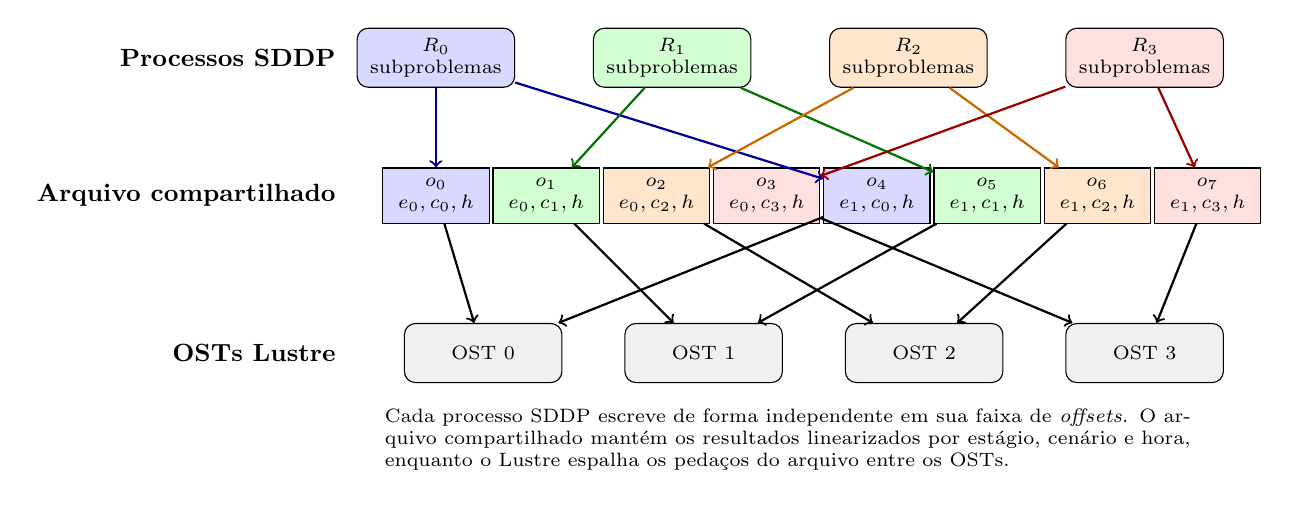
\begin{tikzpicture}[
    font=\scriptsize,
    proc/.style={draw, rounded corners, minimum width=2.0cm, minimum height=0.75cm, align=center},
    seg/.style={draw, minimum width=1.35cm, minimum height=0.7cm, align=center},
    ost/.style={draw, rounded corners, minimum width=2.0cm, minimum height=0.75cm, align=center},
    arr/.style={->, thick}
  ]
    \node[anchor=east, font=\small\bfseries] at (-1.15,2.3) {Processos SDDP};
    \node[proc, fill=blue!15]   (p0) at (0.0,2.3)  {$R_0$\\subproblemas};
    \node[proc, fill=green!18]  (p1) at (3.0,2.3)  {$R_1$\\subproblemas};
    \node[proc, fill=orange!20] (p2) at (6.0,2.3)  {$R_2$\\subproblemas};
    \node[proc, fill=red!12]    (p3) at (9.0,2.3)  {$R_3$\\subproblemas};

    \node[anchor=east, font=\small\bfseries] at (-1.15,0.55)
      {Arquivo compartilhado};
    \node[seg, fill=blue!15]   (f0) at (0.0,0.55) {$o_0$\\$e_0,c_0,h$};
    \node[seg, fill=green!18]  (f1) at (1.4,0.55) {$o_1$\\$e_0,c_1,h$};
    \node[seg, fill=orange!20] (f2) at (2.8,0.55) {$o_2$\\$e_0,c_2,h$};
    \node[seg, fill=red!12]    (f3) at (4.2,0.55) {$o_3$\\$e_0,c_3,h$};
    \node[seg, fill=blue!15]   (f4) at (5.6,0.55) {$o_4$\\$e_1,c_0,h$};
    \node[seg, fill=green!18]  (f5) at (7.0,0.55) {$o_5$\\$e_1,c_1,h$};
    \node[seg, fill=orange!20] (f6) at (8.4,0.55) {$o_6$\\$e_1,c_2,h$};
    \node[seg, fill=red!12]    (f7) at (9.8,0.55) {$o_7$\\$e_1,c_3,h$};

    \draw[arr, blue!60!black]   (p0) -- (f0);
    \draw[arr, blue!60!black]   (p0) -- (f4);
    \draw[arr, green!45!black]  (p1) -- (f1);
    \draw[arr, green!45!black]  (p1) -- (f5);
    \draw[arr, orange!80!black] (p2) -- (f2);
    \draw[arr, orange!80!black] (p2) -- (f6);
    \draw[arr, red!60!black]    (p3) -- (f3);
    \draw[arr, red!60!black]    (p3) -- (f7);

    \node[anchor=east, font=\small\bfseries] at (-1.15,-1.45) {OSTs Lustre};
    \node[ost, fill=gray!12] (ost0) at (0.6,-1.45) {OST 0};
    \node[ost, fill=gray!12] (ost1) at (3.4,-1.45) {OST 1};
    \node[ost, fill=gray!12] (ost2) at (6.2,-1.45) {OST 2};
    \node[ost, fill=gray!12] (ost3) at (9.0,-1.45) {OST 3};

    \draw[arr] (f0) -- (ost0);
    \draw[arr] (f1) -- (ost1);
    \draw[arr] (f2) -- (ost2);
    \draw[arr] (f3) -- (ost3);
    \draw[arr] (f4) -- (ost0);
    \draw[arr] (f5) -- (ost1);
    \draw[arr] (f6) -- (ost2);
    \draw[arr] (f7) -- (ost3);

    \node[align=left, text width=10.5cm] at (4.6,-2.55) {
      Cada processo SDDP escreve de forma independente em sua faixa de
      \textit{offsets}. O arquivo compartilhado mantém os resultados
      linearizados por estágio, cenário e hora, enquanto o Lustre espalha os
      pedaços do arquivo entre os OSTs.
    };
  \end{tikzpicture}
  }
  \caption{Escrita independente dos processos SDDP em um arquivo compartilhado
  e distribuição dos pedaços em OSTs do Lustre.}
  \label{fig:layout_resultados_lustre}
\end{figure}

\begin{figure}[H]
  \centering
  
\includegraphics[width=0.7\textwidth]{SDDP_architecture2.png}
  \caption{Proposta com MPI-IO e Lustre.}
  \label{fig:SDDP_architecture2}
\end{figure}



%===============================================================================
\chapter{Avaliações}
\label{cap:avaliacoes}

Este capítulo apresenta a avaliação comparativa entre a implementação atual
de entrada e saída (E/S) e a implementação proposta, com o objetivo de
investigar ganhos de desempenho e melhorias de escalabilidade,
principalmente em ambientes de computação em nuvem. A análise concentra-se
em métricas de tempo de execução, tempo de comunicação, largura de banda e
tempo de bloqueio das operações de E/S, considerando o impacto das
estratégias adotadas para operações paralelas de E/S em cenários de alto
desempenho~\cite{Rwe:99,Phrrbrw:09}.

A base de dados utilizada nos experimentos corresponde ao PMO/PAR de
outubro de 2023. Para a etapa de simulação horária, que constitui o foco
principal deste estudo, foram considerados 1.536 cenários em ambos os
experimentos (AWS e SDumont), com três estágios mensais.

Para cada configuração avaliada, foram executadas cinco repetições; os
valores reportados nas tabelas e figuras deste capítulo correspondem à
média e ao desvio padrão dessas amostras.

Como cada \textit{rank} MPI apresentou consumo de memória residente
superior a 8~GB, optou-se, em ambos os experimentos, por mapear apenas
um \textit{rank} por núcleo físico --- isto é, sem o uso do
\textit{hyper-threading}. Essa decisão é imposta pela memória total
disponível por nó: com 384~GB por nó nos dois ambientes, ativar
\textit{hyper-threading} e dobrar o número de \textit{ranks}
ultrapassaria a memória física agregada, inviabilizando a execução. O
número de \textit{ranks} por nó foi, portanto, fixado no número de
núcleos físicos da instância correspondente.

Os experimentos conduzidos neste trabalho caracterizam um cenário de
\textit{strong scaling}, no qual o tamanho do problema permanece fixo
enquanto o número de nós computacionais é progressivamente
aumentado~\cite{Amdahl:67}.
Nesse contexto, o acréscimo de recursos implica na redução do volume de
trabalho por nó, sendo esperado, idealmente, que o tempo total de execução
diminua de forma aproximadamente linear com o aumento do paralelismo. No
entanto, essa tendência teórica pode não se concretizar na prática devido
à presença de gargalos sistêmicos, especialmente aqueles relacionados às
operações de entrada e saída (E/S) e à comunicação entre processos. À
medida que o número de nós cresce, a intensificação da concorrência por
recursos compartilhados --- como o sistema de arquivos e a rede --- pode
introduzir sobrecargas adicionais, limitando a eficiência do escalonamento
e reduzindo os ganhos esperados de desempenho.

O tamanho dos blocos de dados foi considerado um fator determinante para a
análise de desempenho de E/S paralela. A
Figura~\ref{fig:histograma_mensagens} apresenta a distribuição agregada
do tamanho dos blocos de dados observados ao longo do experimento.
Observa-se que a distribuição é dominada por blocos de dados pequenos:
1.801.728 blocos, correspondentes a 80,1\% do total, possuem tamanho de
até 1~KB. As demais faixas concentram 152.082 blocos até 128~KB (6,8\%),
267.264 blocos até 1~MB (11,9\%) e 27.648 blocos até 50~MB (1,2\%).
Esse perfil pode comprometer a escalabilidade, já que operações com
granularidade fina tendem a aumentar a sobrecarga de metadados e a
subutilizar a largura de banda disponível~\cite{Rwe:99,Phrrbrw:09}.
Adicionalmente, será avaliado o tempo de envio dos blocos de dados
agrupados por faixas de tamanho, de forma a analisar o impacto da
granularidade das operações no desempenho da comunicação e da E/S.

\begin{figure}[H]
  \centering
  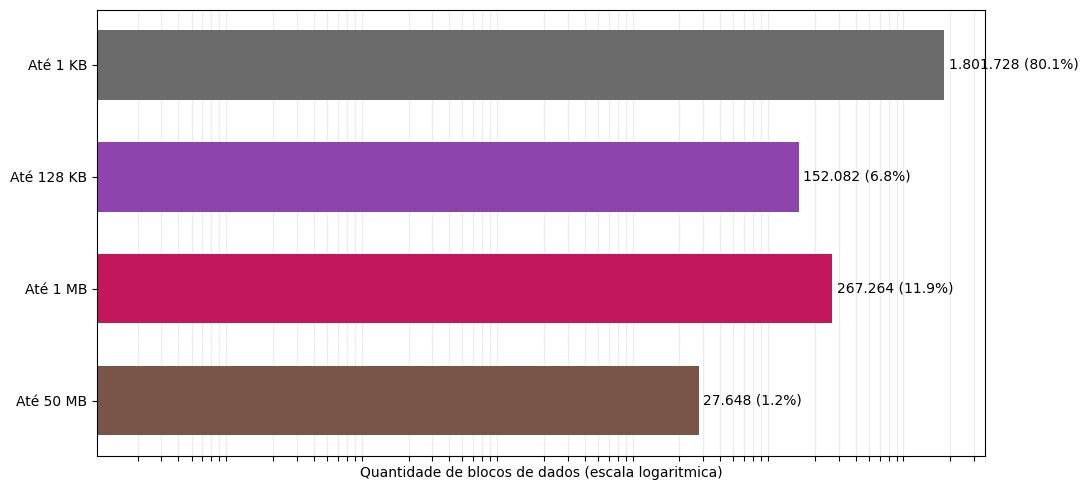
\includegraphics[width=\textwidth]{figuras/histograma_mensagens.png}
  \caption{Distribuição agregada da quantidade de blocos de dados por
  faixa de tamanho no experimento, em escala logarítmica.}
  \label{fig:histograma_mensagens}
\end{figure}

% =============================================================
\section{Experimento AWS}
\label{sec:exp_aws}

O Experimento AWS foi configurado na nuvem da Amazon Web Services (AWS),
utilizando 32 nós da instância do tipo r7i.12xlarge. Essa instância é
baseada na quarta geração de processadores Intel Xeon Scalable (Sapphire
Rapids 8488C), operando a 3,2~GHz, e disponibiliza 24 núcleos físicos com
suporte a \textit{hyper-threading}, totalizando 48 processadores lógicos.
O sistema conta ainda com 384~GB de memória DDR5, que oferece maior
largura de banda em relação às gerações anteriores, e um adaptador de
rede Ethernet com capacidade de até 18,75~Gbps, projetado para cargas de
trabalho intensivas em comunicação. Essa configuração enquadra-se na
categoria de instâncias otimizadas para memória da AWS
(\textit{memory-optimized}), adequada a aplicações que combinam elevada
demanda de processamento paralelo com grandes volumes de dados em
memória --- perfil característico do SDDP, em que cada \textit{rank} MPI
chega a consumir mais de 8~GB de memória residente. Nos experimentos,
utilizou-se a biblioteca MPICH2 versão~3.2 e um sistema de arquivos
paralelo Lustre versão~2.12 de 12~TB, com 1~MDS de 350~GB e 10~OSTs de
1,165~TB. O \textit{stripe count} foi configurado como 10, com
\textit{stripes} de 1~MB, disponibilizado por meio do serviço
Amazon FSx for Lustre. Pelos motivos discutidos na introdução do
capítulo, configurou-se um \textit{rank} por núcleo físico, totalizando
24 \textit{ranks} MPI por nó, que processam cenários em paralelo
segundo o padrão \textit{bag-of-tasks} descrito na
Subseção~\ref{sec:padrao_dados_sddp}~\cite{intel:23,aws:24}.


\subsection{Avaliação da implementação atual}
\label{sec:aws_atual}
Esta subseção analisa o desempenho da arquitetura atual de E/S do SDDP
no Experimento AWS. A Tabela~\ref{tab:central_aws} sumariza os resultados
obtidos com a base de dados PMO/PAR de outubro de 2023, considerando
1.536 cenários, três estágios mensais e 24
\textit{ranks} por nó.

Observa-se que o tempo total de execução cai com o aumento do número de
nós até 16~nós, passando de aproximadamente 8\,971~s em 2~nós para
1\,874~s em 16~nós, mas volta a crescer para 2\,013~s em 32~nós ---
caracterizando o regime saturado típico de um cenário de \textit{strong
scaling} limitado pela E/S. A banda agregada degrada-se de 60{,}5~Gb/s
em 2~nós para 3{,}4~Gb/s em 32~nós (mais de uma ordem de grandeza), e o
percentual do tempo dedicado à E/S cresce de 0{,}34\% em 2~nós para
49{,}51\% em 32~nós. Esses números são coerentes com o
diagnóstico de que o adaptador de rede do nó escritor se torna ponto de
contenção à medida que aumenta o número de processos emissores
concorrentes.

Na Tabela~\ref{tab:central_aws}, o tempo total corresponde ao tempo de
execução medido, que inclui computação, E/S e comunicação. Os tempos de
I/O e comunicação são apresentados separadamente.

\begin{table}[H]
\centering
\caption{Desempenho do Experimento AWS com a implementação atual,
incluindo tempos de I/O, comunicação, tempo total, \textit{speedup},
eficiência e percentual de I/O. A eficiência é calculada em relação à
base de 2~nós.}
\label{tab:central_aws}
\small
\setlength{\tabcolsep}{4pt}
\renewcommand{\arraystretch}{1.25}
\resizebox{\textwidth}{!}{%
\begin{tabular}{cccccccc}
\toprule
\textbf{Nós} &
\textbf{\shortstack{Banda percebida\\(Gb/s)}} &
\textbf{\shortstack{I/O\\(s)}} &
\textbf{\% I/O} &
\textbf{\shortstack{Comunicação\\(s)}} &
\textbf{\shortstack{Total\\(s)}} &
\textbf{Speedup} &
\textbf{\shortstack{Eficiência\\(\%)}} \\
\midrule
2  & $60{,}51 \pm 4{,}56$ & $30{,}85 \pm 2{,}05$ & $0{,}34\%$  & $177{,}51 \pm 26{,}06$ & $8\,971{,}23 \pm 305{,}56$ & $1{,}00\times$ & $100{,}0\%$ \\
4  & $51{,}28 \pm 2{,}48$ & $78{,}23 \pm 3{,}04$ & $1{,}62\%$  & $212{,}76 \pm 16{,}94$ & $4\,823{,}20 \pm 46{,}53$  & $1{,}86\times$ & $93{,}0\%$ \\
8  & $18{,}94 \pm 3{,}30$ & $201{,}67 \pm 4{,}13$ & $7{,}64\%$  & $174{,}04 \pm 11{,}31$ & $2\,639{,}18 \pm 16{,}07$  & $3{,}40\times$ & $85{,}0\%$ \\
16 & $4{,}52  \pm 0{,}29$ & $527{,}94 \pm 2{,}91$ & $28{,}18\%$ & $167{,}77 \pm 6{,}19$  & $1\,873{,}56 \pm 49{,}91$  & $4{,}79\times$ & $59{,}9\%$ \\
32 & $3{,}37  \pm 0{,}09$ & $996{,}57 \pm 5{,}28$ & $49{,}51\%$ & $304{,}96 \pm 3{,}36$  & $2\,013{,}06 \pm 25{,}50$  & $4{,}46\times$ & $27{,}9\%$ \\
\bottomrule
\end{tabular}
}
\end{table}

\subsection{Avaliação da implementação MPI-IO com escritas independentes}
\label{sec:aws_mpiio}
Esta subseção analisa o desempenho da arquitetura proposta, baseada em
escritas independentes com MPI-IO sobre o sistema de arquivos
Lustre, no Experimento AWS. Nesta abordagem cada processo MPI escreve seus
próprios dados diretamente no FSx for Lustre, eliminando o ponto de
contenção associado a um único processo escritor e explorando o
paralelismo dos múltiplos OSTs.

A Tabela~\ref{tab:mpiio_aws} consolida os resultados obtidos com a
implementação MPI-IO no Experimento AWS. Assim como na tabela
anterior, o tempo total corresponde ao tempo de execução medido, que
inclui computação, E/S, comunicação e Coordenação MPI-IO. Os tempos de
I/O, comunicação e Coordenação MPI-IO são apresentados separadamente; a
coordenação corresponde às chamadas
\texttt{MPI\_File\_Open}/\texttt{MPI\_File\_Close}.

\begin{table}[H]
\centering
\caption{Desempenho do Experimento AWS com a implementação MPI-IO,
incluindo tempos de I/O, comunicação, coordenação, tempo total,
\textit{speedup}, eficiência e percentual de I/O. A eficiência é
calculada em relação à base de 2~nós.}
\label{tab:mpiio_aws}
\small
\setlength{\tabcolsep}{4pt}
\renewcommand{\arraystretch}{1.25}
\resizebox{\textwidth}{!}{%
\begin{tabular}{ccccccccc}
\toprule
\textbf{Nós} &
\textbf{\shortstack{Banda percebida\\(Gb/s)}} &
\textbf{\shortstack{I/O\\(s)}} &
\textbf{\% I/O} &
\textbf{\shortstack{Comunicação\\(s)}} &
\textbf{\shortstack{Coord.\\(s)}} &
\textbf{\shortstack{Total\\(s)}} &
\textbf{Speedup} &
\textbf{\shortstack{Eficiência\\(\%)}} \\
\midrule
2  & $57{,}04 \pm 7{,}42$   & $18{,}57 \pm 0{,}86$ & $0{,}21\%$ & $188{,}65 \pm 22{,}49$ & $42{,}48 \pm 6{,}74$  & $8\,858{,}91 \pm 97{,}68$ & $1{,}00\times$ & $100{,}0\%$ \\
4  & $106{,}04 \pm 17{,}02$ & $12{,}54 \pm 0{,}38$ & $0{,}24\%$ & $233{,}95 \pm 21{,}24$ & $51{,}23 \pm 13{,}28$ & $5\,127{,}24 \pm 94{,}25$ & $1{,}73\times$ & $86{,}4\%$ \\
8  & $167{,}03 \pm 35{,}23$ & $9{,}36 \pm 0{,}32$  & $0{,}36\%$ & $186{,}69 \pm 18{,}47$ & $69{,}82 \pm 4{,}10$  & $2\,599{,}75 \pm 32{,}55$ & $3{,}41\times$ & $85{,}2\%$ \\
16 & $274{,}24 \pm 13{,}44$ & $7{,}42 \pm 0{,}10$  & $0{,}48\%$ & $233{,}77 \pm 4{,}50$  & $83{,}53 \pm 3{,}65$  & $1\,558{,}33 \pm 8{,}23$  & $5{,}68\times$ & $71{,}1\%$ \\
32 & $380{,}30 \pm 26{,}86$ & $8{,}93 \pm 0{,}08$  & $0{,}70\%$ & $236{,}02 \pm 8{,}15$  & $147{,}26 \pm 6{,}41$ & $1\,274{,}25 \pm 20{,}95$ & $6{,}95\times$ & $43{,}5\%$ \\
\bottomrule
\end{tabular}
}
\end{table}

\subsection{Análise comparativa}
\label{sec:avaliacao_comparativa_aws}
Os resultados das duas subseções anteriores são consolidados visualmente
nas figuras a seguir, que apresentam, lado a lado, os perfis de banda
agregada, tempo de execução e tempo de bloqueio de envio em função do
número de nós para as duas implementações.

A Tabela~\ref{tab:comparativo_aws} resume os principais indicadores
comparativos do Experimento AWS. A melhoria no tempo total é pequena em
2~nós, torna-se negativa em 4~nós, mas passa a ser positiva a partir de
8~nós e cresce nas maiores escalas: 1{,}5\% em 8~nós, 16{,}8\% em
16~nós e 36{,}7\% em 32~nós. A comparação de banda evidencia o principal
ganho da arquitetura proposta: a MPI-IO passa de desempenho
ligeiramente inferior em 2~nós para 2{,}07$\times$ a banda da
implementação atual em 4~nós, 8{,}82$\times$ em 8~nós, 60{,}66$\times$
em 16~nós e 113{,}00$\times$ em 32~nós. A redução do tempo de E/S também
cresce com a escala, chegando a 99{,}1\% em 32~nós.

\begin{table}[H]
\centering
\caption{Resumo comparativo entre a implementação atual e MPI-IO no
Experimento AWS. A melhoria no total e a melhoria de I/O são calculadas
em relação à implementação atual; valores negativos indicam piora.}
\label{tab:comparativo_aws}
\small
\setlength{\tabcolsep}{3pt}
\renewcommand{\arraystretch}{1.25}
\resizebox{\textwidth}{!}{%
\begin{tabular}{cccccccccc}
\toprule
\textbf{Nós} &
\textbf{\shortstack{Total\\atual (s)}} &
\textbf{\shortstack{Total\\MPI-IO (s)}} &
\textbf{\shortstack{Melhoria\\no total (\%)}} &
\textbf{\shortstack{Banda percebida\\atual (Gb/s)}} &
\textbf{\shortstack{Banda percebida\\MPI-IO (Gb/s)}} &
\textbf{\shortstack{Ganho de\\banda perc.}} &
\textbf{\shortstack{I/O\\atual (s)}} &
\textbf{\shortstack{I/O\\MPI-IO (s)}} &
\textbf{\shortstack{Melhoria\\I/O (\%)}} \\
\midrule
2  & $8\,971{,}23$ & $8\,858{,}91$ & $1{,}3\%$   & $60{,}51$ & $57{,}04$  & $0{,}94\times$   & $30{,}85$  & $18{,}57$ & $39{,}8\%$ \\
4  & $4\,823{,}20$ & $5\,127{,}24$ & $-6{,}3\%$  & $51{,}28$ & $106{,}04$ & $2{,}07\times$   & $78{,}23$  & $12{,}54$ & $84{,}0\%$ \\
8  & $2\,639{,}18$ & $2\,599{,}75$ & $1{,}5\%$   & $18{,}94$ & $167{,}03$ & $8{,}82\times$   & $201{,}67$ & $9{,}36$  & $95{,}4\%$ \\
16 & $1\,873{,}56$ & $1\,558{,}33$ & $16{,}8\%$  & $4{,}52$  & $274{,}24$ & $60{,}66\times$  & $527{,}94$ & $7{,}42$  & $98{,}6\%$ \\
32 & $2\,013{,}06$ & $1\,274{,}25$ & $36{,}7\%$  & $3{,}37$  & $380{,}30$ & $113{,}00\times$ & $996{,}57$ & $8{,}93$  & $99{,}1\%$ \\
\bottomrule
\end{tabular}
}
\end{table}

A Figura~\ref{fig:Banda_AWS} apresenta a evolução da banda agregada
média percebida pela aplicação no Experimento AWS. As duas curvas exibem comportamentos
qualitativamente opostos: a
implementação atual parte de aproximadamente 60{,}5~Gb/s em 2~nós
e degrada-se de forma acentuada com o aumento do paralelismo, atingindo
18{,}9~Gb/s em 8~nós, 4{,}5~Gb/s em 16~nós e 3{,}4~Gb/s em 32~nós ---
uma redução de mais de uma ordem de grandeza. Em contraste, a
implementação MPI-IO parte de 57{,}0~Gb/s em 2~nós e cresce
monotonicamente, alcançando 106{,}0~Gb/s em 4~nós, 167{,}0~Gb/s em
8~nós, 274{,}2~Gb/s em 16~nós e 380{,}3~Gb/s em 32~nós.

Em 2~nós, a banda agregada da implementação atual é cerca de 6\% maior
que a da implementação MPI-IO. Esse comportamento é coerente com o fato
de que, em pequena escala, o gargalo do processo escritor único ainda não
se manifesta, e o custo fixo da coordenação da E/S paralela tem maior
peso relativo. A partir de 4~nós, entretanto, a implementação MPI-IO já
supera a atual. Em 8~nós, a banda agregada é aproximadamente
$8{,}8\times$ maior; em 16~nós, cerca de $60{,}7\times$ maior; e, em
32~nós, aproximadamente $113{,}0\times$ maior. Esse resultado indica que a
arquitetura proposta explora a infraestrutura de armazenamento em uma
escala completamente diferente da arquitetura baseada em escritor único.

Essa diferença de comportamento decorre diretamente da eliminação do
processo escritor único. Na arquitetura atual, todas as escritas
convergem para o adaptador de rede de um único nó, que rapidamente se
torna ponto de contenção e limita o \textit{throughput} global ---
explicando a queda contínua da banda observada. Na abordagem MPI-IO, as operações de escrita são distribuídas entre os
processos MPI, permitindo que múltiplos fluxos de dados sejam enviados
simultaneamente ao sistema de arquivos Lustre, explorando o paralelismo
proporcionado pelos múltiplos OSTs. Como consequência, a banda agregada
cresce de forma consistente com o número de nós, demonstrando que o
sistema de armazenamento ainda não atingiu seu limite nominal na maior
configuração avaliada. Dessa forma, a figura evidencia que a adoção de
MPI-IO não apenas elimina o gargalo da arquitetura atual, mas também
permite um uso significativamente mais eficiente da largura de banda
disponível, tornando a aplicação adequada para execuções em larga escala.

\begin{figure}[H]
  \centering
  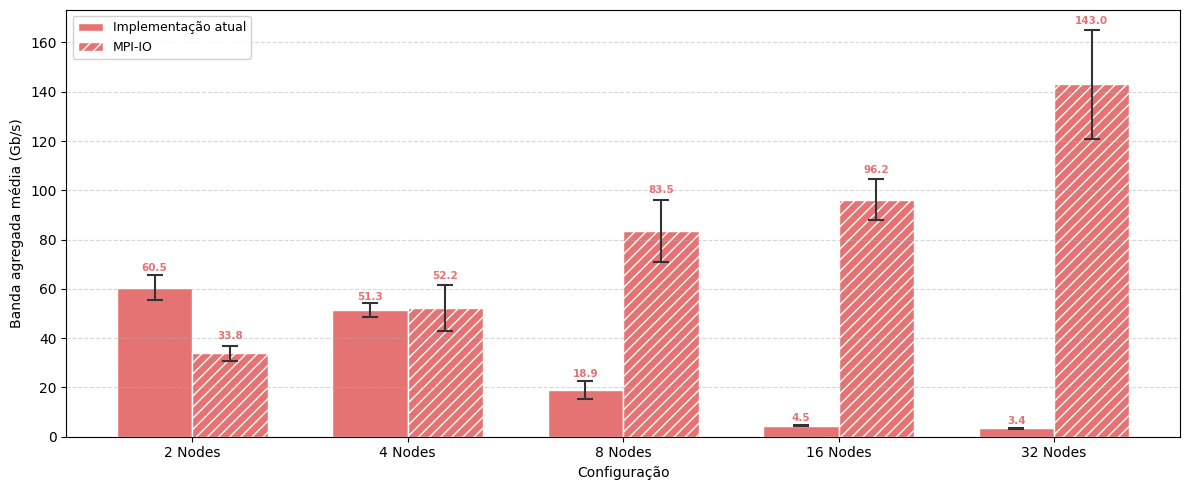
\includegraphics[width=\textwidth]{figuras/Banda_AWS.png}
  \caption{Banda agregada média percebida pela aplicação no
  Experimento AWS.}
  \label{fig:Banda_AWS}
\end{figure}

A Figura~\ref{fig:Tempo_execucao_AWS} apresenta a evolução do tempo total
de execução no Experimento AWS, contrastando a implementação atual e a
implementação MPI-IO sobre o Lustre.
As barras de erro representam apenas o desvio padrão do tempo de execução
total, e não desvios individuais das parcelas internas.
Nas configurações de menor escala, em que a E/S não é o componente
dominante, as duas curvas evoluem de forma próxima: em 2~nós,
$8{,}97 \times 10^{3}$~s no modelo atual contra $8{,}86 \times
10^{3}$~s no modelo MPI-IO; em 4~nós, entretanto, a versão MPI-IO
apresenta $5{,}13 \times 10^{3}$~s contra $4{,}82 \times
10^{3}$~s da implementação atual. Esse comportamento é coerente, uma vez
que, em pequena escala, o tempo de execução é dominado pela computação e
o custo da coordenação ainda tem maior peso relativo.

A divergência entre as duas curvas torna-se evidente a partir de 8~nós e
se acentua de forma marcante nas configurações de maior porte. Enquanto a
implementação atual apresenta um regime de saturação --- com o
tempo de execução passando de $2{,}64 \times 10^{3}$~s em 8~nós para
$1{,}87 \times 10^{3}$~s em 16~nós e voltando a crescer para
$2{,}01 \times 10^{3}$~s em 32~nós ---, a implementação MPI-IO mantém
uma redução consistente do tempo total, atingindo $2{,}60 \times
10^{3}$~s em 8~nós, $1{,}56 \times 10^{3}$~s em 16~nós e $1{,}27
\times 10^{3}$~s em 32~nós. Em termos relativos, isso corresponde a uma
redução do tempo total de aproximadamente 1{,}5\% em 8~nós, 16{,}8\% em
16~nós e 36{,}7\% em 32~nós em relação ao modelo atual.

A figura também evidencia que, na implementação atual, o
crescimento do número de nós deixa de produzir ganho de desempenho a
partir de 16~nós e passa a ser, na prática, contraproducente em 32~nós
--- comportamento característico de regime degradado sob \textit{strong
scaling}, no qual a contenção do processo escritor mais do que compensa
os ganhos de paralelismo computacional. Em contraste, a curva
MPI-IO permanece monotonicamente decrescente em todo o intervalo
avaliado, indicando que a infraestrutura de armazenamento ainda não
atingiu sua capacidade limite mesmo na maior configuração testada.

Cabe observar que, na implementação MPI-IO, o tempo de E/S torna-se uma
fração pequena do tempo total em todas as escalas, permanecendo próximo
ou abaixo de 1\% a partir de 4~nós. Na implementação atual, por outro lado, a
fração de E/S cresce de 7,6\% em 8~nós para 28,2\% em 16~nós e 49,5\%
em 32~nós. Na implementação MPI-IO, parte do tempo de simulação passa a
ser ocupada pela Coordenação MPI-IO, medida pelas chamadas
\texttt{MPI\_File\_Open}/\texttt{MPI\_File\_Close}: essa parcela cresce
de 0{,}5\% em 2~nós para 1{,}0\% em 4~nós, 2{,}7\% em 8~nós, 5{,}4\%
em 16~nós e 11{,}6\% em 32~nós. Esse crescimento percentual, contudo, reflete
sobretudo a redução do tempo de simulação com o aumento do paralelismo
e não um aumento da carga útil tratada por essas chamadas. Como
\texttt{MPI\_File\_Open}/\texttt{MPI\_File\_Close} são executadas
uma única vez por execução --- no início e no final ---, trata-se de
um \emph{overhead fixo} em relação à carga útil do problema: não
cresce com o número de cenários nem com o número de estágios
resolvidos. Esse custo, no entanto, varia com o número de nós
computacionais, já que envolve sincronização coletiva entre todos os
\textit{ranks} envolvidos na abertura do arquivo compartilhado --- e
é exatamente esse comportamento que se observa nos dados, com a
parcela absoluta crescendo de 42~s em 2~nós para 147~s em 32~nós.
Os experimentos aqui apresentados consideram
apenas três estágios mensais, o que mantém o tempo total de
simulação relativamente curto e infla a fração percentual da
Coordenação MPI-IO; em execuções de operação programada típicas do
SIN, com horizonte de vários anos e número de cenários muito maior,
o custo absoluto dessas chamadas, para uma dada configuração de nós,
permanece o mesmo enquanto o tempo total cresce em ordem de
magnitude, diluindo a parcela de coordenação para níveis
desprezíveis. A partir de 8~nós, e mesmo sob essa inflação relativa do
custo de coordenação, a implementação MPI-IO já apresenta
tempo total inferior ao da implementação atual.

\begin{figure}[H]
  \centering
  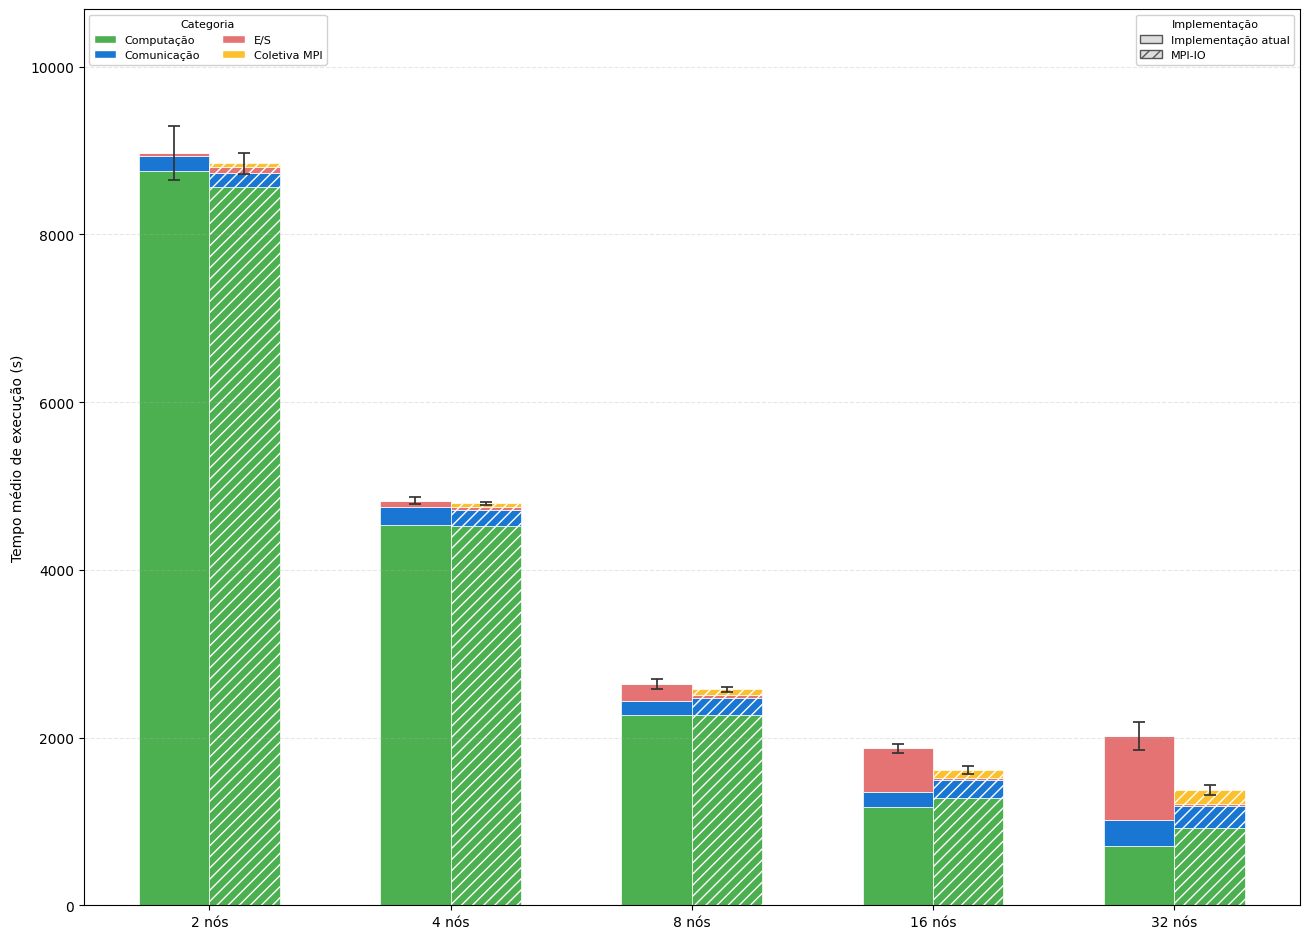
\includegraphics[width=\textwidth]{figuras/Tempo_execucao_AWS.png}
  \caption{Tempo de execução no Experimento AWS.}
  \label{fig:Tempo_execucao_AWS}
\end{figure}

A Figura~\ref{fig:EnvioPorTamanho_AWS} apresenta o tempo médio de
bloqueio das operações de E/S, em segundos, em função do tamanho dos
blocos de dados no Experimento AWS, em escala logarítmica. A comparação mostra
que, para blocos de dados muito pequenos, a implementação atual apresenta
tempos menores, pois o custo fixo das chamadas MPI-IO se torna dominante em
relação ao volume transferido. Esse efeito, contudo, ocorre em uma faixa de
tempo baixa, da ordem de microssegundos a poucos milissegundos, e não
determina o tempo total da aplicação.

Para blocos de dados médios e grandes, que concentram o impacto de E/S nas
maiores escalas, o comportamento se inverte. Em 16 e 32~nós, a
implementação atual passa a apresentar tempos de bloqueio elevados nas
classes de maior tamanho, chegando à ordem de segundos, enquanto a
implementação MPI-IO permanece na ordem de centésimos ou décimos de segundo.
Assim, a figura reforça o diagnóstico das Figuras~\ref{fig:Banda_AWS}
e~\ref{fig:Tempo_execucao_AWS}: a abordagem com escritor único é competitiva
apenas em pequena escala ou para blocos de dados muito pequenos, mas perde
escalabilidade quando o volume de dados e a concorrência entre processos
aumentam.

\begin{figure}[H]
  \centering
  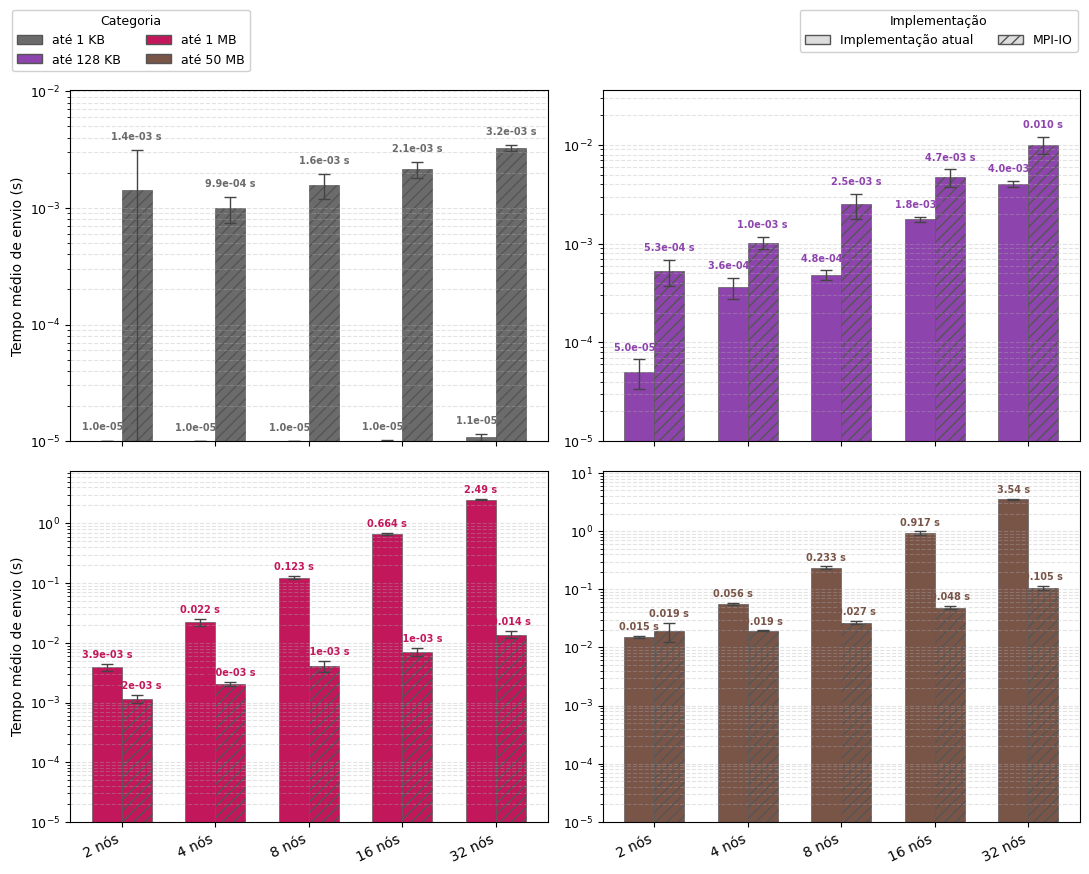
\includegraphics[width=\textwidth]{figuras/EnvioPorTamanho_AWS.png}
  \caption{Tempo médio de bloqueio das operações de envio em função do
  tamanho dos blocos de dados no Experimento AWS (escala logarítmica).}
  \label{fig:EnvioPorTamanho_AWS}
\end{figure}

% =============================================================
\subsection{Avaliação do impacto do número de OSTs}
\label{sec:exp_osts}

Esta subseção tem como objetivo avaliar, no Experimento AWS, o impacto do número de
\textit{Object Storage Targets} (OSTs) no desempenho das operações de E/S
no sistema de arquivos Lustre. Em ambientes HPC, a quantidade de OSTs
está diretamente relacionada ao grau de paralelismo de E/S disponível,
uma vez que os dados podem ser distribuídos entre múltiplos dispositivos
de armazenamento, permitindo acessos concorrentes por diferentes
processos.

A análise apresentada nesta subseção foi conduzida em rodada experimental
específica, com instrumentação dedicada à isolação do efeito do número de
OSTs. Os valores absolutos não devem ser comparados diretamente com os
das Subseções \ref{sec:aws_atual}--\ref{sec:avaliacao_comparativa_aws}
(em particular, com a Tabela~\ref{tab:mpiio_aws}); o foco aqui é a
tendência relativa entre as configurações de 4 e 10 OSTs.

Para esta avaliação, foram realizados experimentos com a abordagem
MPI-IO variando-se a quantidade de OSTs disponíveis no FSx for Lustre,
comparando configurações com 4~OSTs e 10~OSTs para execuções com 16 e
32~nós de cálculo. As demais características do experimento foram
mantidas constantes, incluindo o volume de dados e o padrão de acesso,
de modo a isolar o efeito da infraestrutura de armazenamento.

A Figura~\ref{fig:Experimento_OSTs} apresenta o tempo médio de envio
por classe de tamanho das mensagens. Cada subfigura corresponde a uma
classe de tamanho, enquanto as barras comparam as configurações MPI-IO
com 4 e 10~OSTs para 16 e 32~nós de cálculo. Em 16~nós, o uso de
10~OSTs aumenta o tempo médio de envio nas classes pequenas, de
0{,}014~ms para 2{,}1~ms nas mensagens de até 1~KB e de 0{,}014~ms para
4{,}7~ms nas mensagens de até 128~KB. Nas classes que concentram maior
volume de dados, porém, o comportamento se inverte: o tempo cai de
82{,}6~ms para 7{,}1~ms nas mensagens de até 1~MB e de 524~ms para
48~ms nas mensagens de até 50~MB.

O efeito é mais pronunciado em 32~nós, quando a maior concorrência entre
processos amplia a diferença entre as duas configurações. Nesse cenário,
as classes pequenas permanecem mais rápidas com 4~OSTs, com tempos de
0{,}018~ms nas mensagens de até 1~KB e 0{,}018~ms nas mensagens de até
128~KB, contra 3{,}2~ms e 10~ms com 10~OSTs. Para blocos maiores,
entretanto, o aumento do número de OSTs reduz o tempo médio de envio de
309~ms para 13{,}7~ms nas mensagens de até 1~MB e de 1{,}89~s para
105~ms nas mensagens de até 50~MB. Esses resultados mostram que a
redução do número de OSTs aumenta a contenção no acesso aos dados
principalmente nas classes de maior volume, sobretudo quando o número de
nós de cálculo cresce. Embora a escrita seja realizada em paralelo por
meio de MPI-IO, a disponibilidade de menos alvos de armazenamento limita
o paralelismo efetivo do Lustre e aumenta o tempo observado nas
operações de envio dessas classes.

\begin{figure}[H]
  \centering
  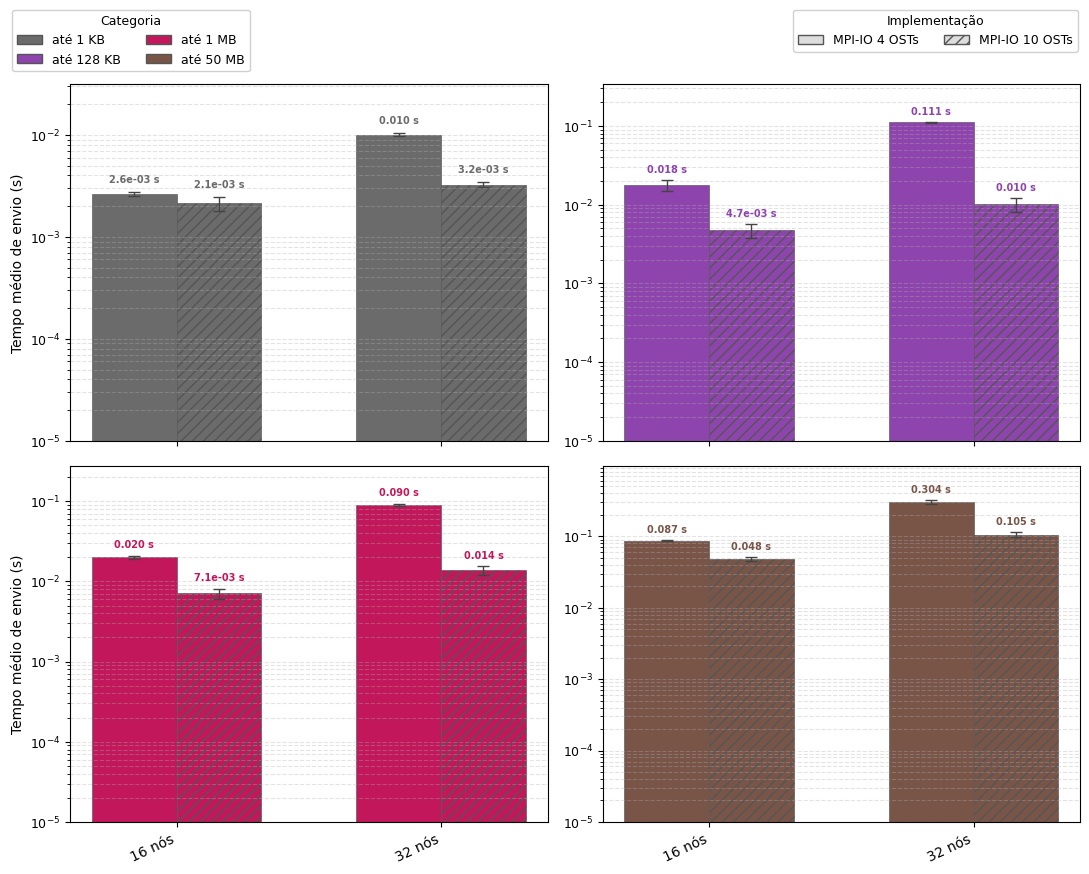
\includegraphics[width=\textwidth]{figuras/Experimento_OSTs.png}
  \caption{Tempo médio de envio por classe de tamanho das mensagens para
  configurações MPI-IO com 4 e 10~OSTs.}
  \label{fig:Experimento_OSTs}
\end{figure}

A Figura~\ref{fig:Experimento_OSTs_banda} complementa essa análise ao
apresentar a banda agregada média percebida pela aplicação em cada
configuração. Com
16~nós, a configuração com 10~OSTs atinge 274{,}2~Gb/s, contra
49{,}4~Gb/s com 4~OSTs, ganho de aproximadamente 5{,}6$\times$. Ao
passar de 16 para 32~nós, as configurações exibem tendências opostas:
com 10~OSTs, a banda cresce para 380{,}3~Gb/s, enquanto, com 4~OSTs, cai
para 16{,}1~Gb/s. Dessa forma, em 32~nós, o uso de 10~OSTs resulta em
ganho de aproximadamente 23{,}6$\times$ sobre a configuração com 4~OSTs.
Esse comportamento indica que, quando a concorrência entre processos
aumenta, a configuração com menos OSTs passa a limitar a escalabilidade
da E/S.

Assim, a análise conjunta das duas figuras indica que o aumento no
número de OSTs melhora tanto a largura de banda agregada quanto o tempo
médio das operações de envio nas classes de maior volume. A configuração
com 10~OSTs permite melhor distribuição das requisições entre os alvos de
armazenamento, enquanto a configuração com 4~OSTs concentra o tráfego em
menos dispositivos e introduz gargalos mais visíveis no cenário com
32~nós.

\begin{figure}[H]
  \centering
  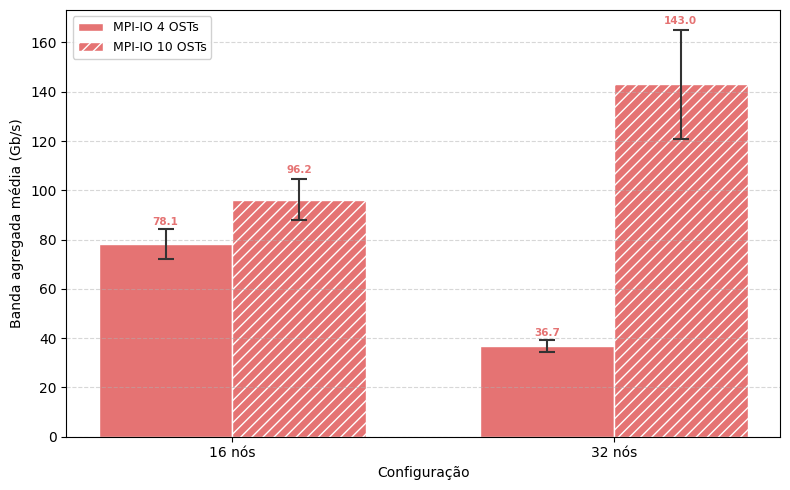
\includegraphics[width=\textwidth]{figuras/Experimento_OSTs_banda.png}
  \caption{Banda agregada média percebida pela aplicação na
  implementação MPI-IO para configurações com 4 e 10~OSTs em 16 e
  32~nós.}
  \label{fig:Experimento_OSTs_banda}
\end{figure}

% =============================================================
\section{Experimento SDumont}
\label{sec:exp_sdumont}

O Experimento SDumont corresponde ao supercomputador Santos Dumont
(SDumont), adquirido junto à empresa francesa EVIDEN/ATOS/BULL, que está
localizado na sede do Laboratório Nacional de Computação Científica
(LNCC), em Petrópolis-RJ, atuando como nó central (Tier-0) do Sistema
Nacional de Processamento de Alto Desempenho (SINAPAD). Nesse experimento
foram utilizados até 32~nós de processamento, cada um equipado com dois
processadores Intel Xeon Cascade Lake Gold 6252, totalizando 24~núcleos
físicos por nó, com suporte a \textit{hyper-threading}, o que resulta em
48~processadores lógicos disponíveis. Cada nó conta ainda com 384~GB de
memória e interconexão de alta velocidade baseada em InfiniBand EDR de
100~Gb/s, projetada para reduzir a latência e aumentar a eficiência em
aplicações paralelas de larga escala. Nos experimentos, foi utilizada a
biblioteca MPICH2 versão~3.2 e um sistema de arquivos paralelo Lustre
v2.12 implementado através do ClusterStor L300 da Cray/HPE. Essa
implementação do Lustre é composta por 1~nó MDS (com 1~MDT) e 6~nós OSSs
(cada um servindo 1~OST). O \textit{stripe count} foi configurado como 6,
com \textit{stripes} de 1~MB, disponibilizando um
espaço total de armazenamento de 1,1~PB. Pelos motivos discutidos na
introdução do capítulo, também aqui se configurou um \textit{rank} por
núcleo físico, totalizando 24 \textit{ranks} MPI por nó, que processam
cenários em paralelo segundo o padrão \textit{bag-of-tasks}.

Diferentemente do FSx for Lustre dedicado utilizado no Experimento AWS, o
sistema de arquivos do SDumont é compartilhado com outras cargas de
trabalho de HPC executando concorrentemente, o que introduz variabilidade
adicional nas medições e amplifica o efeito da contenção sobre os
recursos do sistema de arquivos nas maiores escalas. Esse compartilhamento
faz do SDumont um cenário mais desafiador para a avaliação da
escalabilidade de E/S do que o ambiente isolado da AWS.


\subsection{Avaliação da implementação atual}
\label{sec:sdumont_atual}
Esta subseção analisa o desempenho da arquitetura atual de E/S do SDDP
no Experimento SDumont. A Tabela~\ref{tab:central_sdumont} sumariza os
resultados, considerando 1.536 cenários, três estágios mensais e 24
\textit{ranks} por nó.

O tempo total de execução medido decresce com o
aumento do número de nós: 14.703~s em 2~nós, 7.572~s em 4~nós,
4.987~s em 8~nós, 2.993~s em 16~nós e 2.989~s em 32~nós. Essa redução,
contudo, perde eficiência rapidamente: o speedup passa de
1{,}94$\times$ em 4~nós para 2{,}95$\times$ em 8~nós,
4{,}91$\times$ em 16~nós e 4{,}92$\times$ em 32~nós, o que corresponde
a queda de eficiência de 97{,}1\% para 30{,}7\%. Notavelmente, o tempo
total praticamente estagna entre 16 e 32~nós (2.993~s e 2.989~s,
respectivamente), sintoma de que o gargalo da arquitetura
centralizada já se manifesta a partir de 16~nós e impede ganhos
adicionais com o aumento do paralelismo. A banda agregada percebida
confirma o diagnóstico: parte de 62{,}8~Gb/s em 2~nós, recua para
46{,}2~Gb/s em 4~nós e colapsa a partir de 8~nós, mantendo-se entre
3{,}8 e 5{,}4~Gb/s no restante da faixa avaliada. A parcela de E/S,
embutida no tempo de simulação, salta de 0{,}24\% em 2~nós para
19{,}43\% em 8~nós, 21{,}85\% em 16~nós e 39{,}98\% em 32~nós,
evidência direta de que o gargalo da arquitetura centralizada se
intensifica nas maiores escalas.

\begin{table}[H]
\centering
\caption{Desempenho do Experimento SDumont com a implementação atual. O
tempo total corresponde ao tempo de execução medido, que inclui computação,
E/S e comunicação. A eficiência é calculada em relação à base de 2~nós.}
\label{tab:central_sdumont}
\small
\setlength{\tabcolsep}{4pt}
\renewcommand{\arraystretch}{1.25}
\resizebox{\textwidth}{!}{%
\begin{tabular}{cccccccc}
\toprule
\textbf{Nós} &
\textbf{\shortstack{Banda percebida\\(Gb/s)}} &
\textbf{\shortstack{I/O\\(s)}} &
\textbf{\% I/O} &
\textbf{\shortstack{Comunicação\\(s)}} &
\textbf{\shortstack{Total\\(s)}} &
\textbf{Speedup} &
\textbf{\shortstack{Eficiência\\(\%)}} \\
\midrule
2  & $62{,}78 \pm 1{,}83$ & $34{,}73 \pm 1{,}01$       & $0{,}24\%$  & $374{,}04 \pm 13{,}10$ & $14\,702{,}88 \pm 26{,}41$ & $1{,}00\times$ & $100{,}0\%$ \\
4  & $46{,}19 \pm 3{,}15$ & $75{,}76 \pm 2{,}59$       & $1{,}00\%$  & $332{,}55 \pm 12{,}98$ & $7\,571{,}66 \pm 14{,}39$  & $1{,}94\times$ & $97{,}1\%$ \\
8  & $4{,}26 \pm 0{,}29$  & $968{,}97 \pm 6{,}94$      & $19{,}43\%$ & $385{,}68 \pm 19{,}75$ & $4\,987{,}34 \pm 77{,}08$  & $2{,}95\times$ & $73{,}7\%$ \\
16 & $5{,}37 \pm 0{,}87$  & $654{,}04 \pm 3{,}73$      & $21{,}85\%$ & $395{,}28 \pm 9{,}54$  & $2\,992{,}77 \pm 77{,}20$  & $4{,}91\times$ & $61{,}4\%$ \\
32 & $3{,}77 \pm 1{,}02$  & $1\,194{,}97 \pm 7{,}10$   & $39{,}98\%$ & $494{,}93 \pm 15{,}30$ & $2\,988{,}68 \pm 75{,}36$  & $4{,}92\times$ & $30{,}7\%$ \\
\bottomrule
\end{tabular}
}
\end{table}

\subsection{Avaliação da implementação MPI-IO com escritas independentes}
\label{sec:sdumont_mpiio}
Esta subseção analisa o desempenho da arquitetura proposta no
Experimento SDumont, baseada em escritas independentes com MPI-IO sobre o
sistema de arquivos Lustre operado pelo ClusterStor L300. A
Tabela~\ref{tab:mpiio_sdumont} consolida os resultados.

Na implementação MPI-IO, o tempo total decresce ao longo de toda a
faixa avaliada: 15.096~s em 2~nós, 7.912~s em 4~nós, 4.151~s em
8~nós, 2.619~s em 16~nós e 2.133~s em 32~nós. Em comparação com a
implementação atual, a versão MPI-IO apresenta pequeno sobrecusto em
2 e 4~nós (aumento de 2{,}7\% e 4{,}5\%, respectivamente), mas passa
a reduzir o tempo total a partir de 8~nós, com ganhos de 16{,}8\%,
12{,}5\% e 28{,}6\% em 8, 16 e 32~nós. A banda agregada do
\textit{layer} de escrita, ao contrário do que ocorre na implementação
atual, cresce de forma consistente com o paralelismo: de 5{,}5~Gb/s
em 2~nós para 8{,}9~Gb/s em 4~nós, 12{,}1~Gb/s em 8~nós,
18{,}9~Gb/s em 16~nós e 34{,}1~Gb/s em 32~nós. O tempo médio de E/S
por processo cai de 320~s em 2~nós para 61{,}6~s em 32~nós, e a
parcela percentual de E/S no tempo de simulação permanece abaixo de
5\% em todas as configurações.

\begin{table}[H]
\centering
\caption{Desempenho do Experimento SDumont com a implementação MPI-IO. O
tempo total corresponde ao tempo de execução medido, que inclui computação,
E/S, comunicação e Coordenação MPI-IO. A eficiência é calculada em relação
à base de 2~nós.}
\label{tab:mpiio_sdumont}
\small
\setlength{\tabcolsep}{4pt}
\renewcommand{\arraystretch}{1.25}
\resizebox{\textwidth}{!}{%
\begin{tabular}{ccccccccc}
\toprule
\textbf{Nós} &
\textbf{\shortstack{Banda percebida\\(Gb/s)}} &
\textbf{\shortstack{I/O\\(s)}} &
\textbf{\% I/O} &
\textbf{\shortstack{Comunicação\\(s)}} &
\textbf{\shortstack{Coord.\\(s)}} &
\textbf{\shortstack{Total\\(s)}} &
\textbf{Speedup} &
\textbf{\shortstack{Eficiência\\(\%)}} \\
\midrule
2  & $5{,}55 \pm 0{,}33$  & $320{,}27 \pm 10{,}78$ & $2{,}12\%$ & $352{,}81 \pm 7{,}54$  & $23{,}24 \pm 2{,}65$   & $15\,096{,}47 \pm 40{,}60$  & $1{,}00\times$ & $100{,}0\%$ \\
4  & $8{,}89 \pm 0{,}85$  & $270{,}52 \pm 4{,}45$  & $3{,}42\%$ & $231{,}00 \pm 11{,}26$ & $32{,}27 \pm 1{,}40$   & $7\,912{,}23 \pm 81{,}80$   & $1{,}91\times$ & $95{,}4\%$ \\
8  & $12{,}09 \pm 1{,}33$ & $193{,}57 \pm 2{,}23$  & $4{,}66\%$ & $222{,}57 \pm 6{,}92$  & $79{,}31 \pm 19{,}18$  & $4\,151{,}01 \pm 124{,}19$  & $3{,}64\times$ & $90{,}9\%$ \\
16 & $18{,}85 \pm 1{,}04$ & $99{,}41 \pm 0{,}95$   & $3{,}79\%$ & $281{,}28 \pm 16{,}08$ & $126{,}49 \pm 24{,}82$ & $2\,619{,}43 \pm 88{,}31$   & $5{,}76\times$ & $72{,}0\%$ \\
32 & $34{,}10 \pm 4{,}70$ & $61{,}61 \pm 0{,}78$   & $2{,}89\%$ & $357{,}72 \pm 19{,}57$ & $230{,}03 \pm 7{,}78$  & $2\,132{,}82 \pm 75{,}89$   & $7{,}08\times$ & $44{,}2\%$ \\
\bottomrule
\end{tabular}
}
\end{table}

\subsection{Análise comparativa}
\label{sec:avaliacao_comparativa_sdumont}
Os resultados das duas subseções anteriores são consolidados visualmente
nas figuras a seguir, que apresentam, lado a lado, os perfis de banda
agregada, tempo de execução e tempo de bloqueio de envio em função do
número de nós para as duas implementações no Experimento SDumont.

A Tabela~\ref{tab:comparativo_sdumont} resume os principais indicadores
comparativos do Experimento SDumont. A coluna de melhoria no tempo total
compara diretamente a implementação MPI-IO com a implementação atual para
o mesmo número de nós, calculada como
$(Total_{atual} - Total_{MPIIO})/Total_{atual}$. Valores positivos
indicam redução do tempo total, enquanto valores negativos indicam piora.
A MPI-IO apresenta sobrecusto em pequena escala (--2{,}7\% em 2~nós e
--4{,}5\% em 4~nós), mas passa a reduzir o tempo total a partir de
8~nós, com ganhos de 16{,}8\%, 12{,}5\% e 28{,}6\% em 8, 16 e
32~nós. O ganho de banda também cresce nas maiores escalas: alcança
2{,}83$\times$ em 8~nós, 3{,}51$\times$ em 16~nós e 9{,}05$\times$
em 32~nós. A redução do tempo médio de E/S chega a 80{,}0\% em
8~nós, 84{,}8\% em 16~nós e 94{,}8\% em 32~nós, atestando que a
contenção do escritor único é o fator dominante de degradação da
implementação atual nessas escalas.

\begin{table}[H]
\centering
\caption{Resumo comparativo entre a implementação atual e MPI-IO no
Experimento SDumont. A melhoria no total e a melhoria de I/O são
calculadas em relação à implementação atual; valores negativos indicam
piora.}
\label{tab:comparativo_sdumont}
\small
\setlength{\tabcolsep}{3pt}
\renewcommand{\arraystretch}{1.25}
\resizebox{\textwidth}{!}{%
\begin{tabular}{cccccccccc}
\toprule
\textbf{Nós} &
\textbf{\shortstack{Total\\atual (s)}} &
\textbf{\shortstack{Total\\MPI-IO (s)}} &
\textbf{\shortstack{Melhoria\\no total (\%)}} &
\textbf{\shortstack{Banda percebida\\atual (Gb/s)}} &
\textbf{\shortstack{Banda percebida\\MPI-IO (Gb/s)}} &
\textbf{\shortstack{Ganho de\\banda perc.}} &
\textbf{\shortstack{I/O\\atual (s)}} &
\textbf{\shortstack{I/O\\MPI-IO (s)}} &
\textbf{\shortstack{Melhoria\\I/O (\%)}} \\
\midrule
2  & $14\,702{,}88$ & $15\,096{,}47$ & $-2{,}7\%$  & $62{,}78$ & $5{,}55$  & $0{,}09\times$ & $34{,}73$  & $320{,}27$ & $-822{,}2\%$ \\
4  & $7\,571{,}66$  & $7\,912{,}23$  & $-4{,}5\%$  & $46{,}19$ & $8{,}89$  & $0{,}19\times$ & $75{,}76$  & $270{,}52$ & $-257{,}1\%$ \\
8  & $4\,987{,}34$  & $4\,151{,}01$  & $16{,}8\%$  & $4{,}26$  & $12{,}09$ & $2{,}83\times$ & $968{,}97$ & $193{,}57$ & $80{,}0\%$ \\
16 & $2\,992{,}77$  & $2\,619{,}43$  & $12{,}5\%$  & $5{,}37$  & $18{,}85$ & $3{,}51\times$ & $654{,}04$ & $99{,}41$  & $84{,}8\%$ \\
32 & $2\,988{,}68$  & $2\,132{,}82$  & $28{,}6\%$  & $3{,}77$  & $34{,}10$ & $9{,}05\times$ & $1\,194{,}97$ & $61{,}61$  & $94{,}8\%$ \\
\bottomrule
\end{tabular}
}
\end{table}

A Figura~\ref{fig:Banda_SDumont} compara a banda agregada média
percebida pela aplicação
obtida pela implementação atual e pela implementação MPI-IO. Em 2 e
4~nós, a implementação atual apresenta a maior banda observada, com
62{,}8~Gb/s e 46{,}2~Gb/s respectivamente, enquanto a MPI-IO atinge
5{,}5~Gb/s e 8{,}9~Gb/s --- comportamento esperado em pequena
escala, em que o custo fixo da camada MPI-IO ainda não é amortizado
pelo paralelismo de escrita. A partir de 8~nós, o quadro se inverte:
a banda da implementação atual colapsa para 4{,}3~Gb/s e a MPI-IO
sobe para 12{,}1~Gb/s --- ganho de 2{,}83$\times$. Em 16~nós, a
implementação atual permanece nesse patamar baixo, com 5{,}4~Gb/s,
enquanto a MPI-IO continua crescendo e alcança 18{,}9~Gb/s --- ganho
de 3{,}51$\times$. Em 32~nós, a diferença se acentua: a implementação
atual cai para 3{,}8~Gb/s, enquanto a MPI-IO atinge 34{,}1~Gb/s,
ganho de 9{,}05$\times$.

Mais relevante que o valor absoluto é o contraste de
\emph{comportamento}: a implementação atual exibe queda abrupta entre
4 e 8~nós e permanece em um patamar baixo nas escalas subsequentes
(entre 3{,}8 e 5{,}4~Gb/s), sintoma da saturação do escritor central
sob o Lustre compartilhado do SDumont. A implementação MPI-IO, em
contrapartida, apresenta perfil monotonicamente crescente de banda,
indicando que a infraestrutura de armazenamento ainda é capaz de
absorver maior paralelismo de escrita.

\begin{figure}[H]
  \centering
  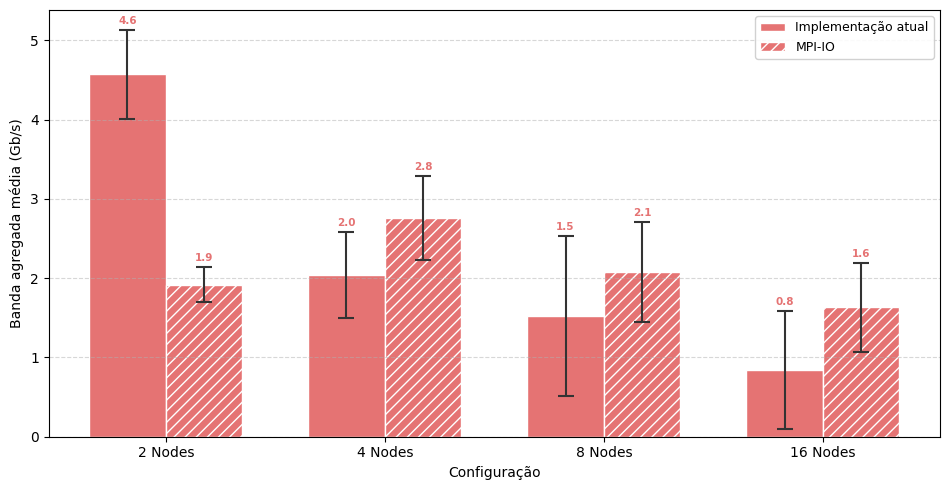
\includegraphics[width=\textwidth]{figuras/Banda_SDumont.png}
  \caption{Banda agregada média percebida pela aplicação nas
  implementações atual e MPI-IO no Experimento SDumont.}
  \label{fig:Banda_SDumont}
\end{figure}

A Figura~\ref{fig:Tempo_execucao_SDumont} detalha o tempo médio por
processo no Experimento SDumont, separando as parcelas de computação,
comunicação, E/S e Coordenação MPI-IO. A parcela Coordenação MPI-IO
corresponde às chamadas
\texttt{MPI\_File\_Open}/\texttt{MPI\_File\_Close}, executadas
\emph{uma única vez} por execução --- na abertura e no fechamento do
arquivo de saída. Trata-se, portanto, de um \emph{overhead fixo} em
relação à carga útil do problema: não cresce com o número de
cenários nem com o número de estágios resolvidos. Esse custo, no
entanto, varia com o número de nós computacionais, já que envolve
sincronização coletiva entre todos os \textit{ranks} envolvidos na
abertura do arquivo compartilhado. As
barras de erro indicam somente o desvio padrão do tempo de execução
total. Em 2 e 4~nós, a implementação MPI-IO apresenta tempo total
levemente superior ao da implementação atual: o custo das operações
de coordenação e da própria camada MPI-IO ainda pesa nessas escalas,
em que a contenção do escritor único da implementação atual ainda
não saturou. A partir de 8~nós, a versão MPI-IO reduz o tempo total
em relação à implementação atual, chegando a 28{,}6\% de redução em
32~nós.

Na implementação atual, a parcela de E/S cresce de forma marcante a
partir de 8~nós, chegando a representar uma fatia significativa do
tempo de simulação. Esse comportamento é compatível com a saturação
do processo escritor centralizado no Lustre compartilhado do
SDumont. Na implementação MPI-IO, o tempo de E/S é redistribuído
entre os processos e permanece reduzido em todas as escalas
(abaixo de 5\% do tempo de simulação), enquanto o custo da
Coordenação MPI-IO passa a compor uma fração visível do tempo total
nas maiores configurações --- em particular, cresce de cerca de
23~s em 2~nós para 126~s em 16~nós e 230~s em 32~nós.

É importante destacar que a fração relativa da Coordenação MPI-IO
observada nestes experimentos é maior do que se espera em execuções
reais do SDDP. Como já discutido, trata-se de um overhead fixo em
relação à carga útil do problema --- não cresce com o número de
cenários nem com o número de estágios resolvidos ---, de modo que
sua participação no tempo total decresce à medida que a carga
computacional aumenta. Nas execuções aqui realizadas, com apenas
três estágios mensais e $1\,536$ cenários, o tempo total de
simulação é relativamente baixo, o que infla o peso percentual dessa
parcela. Em execuções de operação programada típicas do SIN, com
horizonte de vários anos em resolução mensal e número de cenários
muito maior, o custo absoluto de coordenação, para uma dada
configuração de nós, permanece o mesmo enquanto o tempo total de
computação cresce em ordem de magnitude
--- diluindo a fração relativa da Coordenação MPI-IO para níveis
desprezíveis. Assim, a figura evidencia que a abordagem proposta
reduz o gargalo centralizado de escrita; o custo residual de
coordenação, embora visível na escala dos experimentos, não é uma
limitação intrínseca da arquitetura proposta.

\begin{figure}[H]
  \centering
  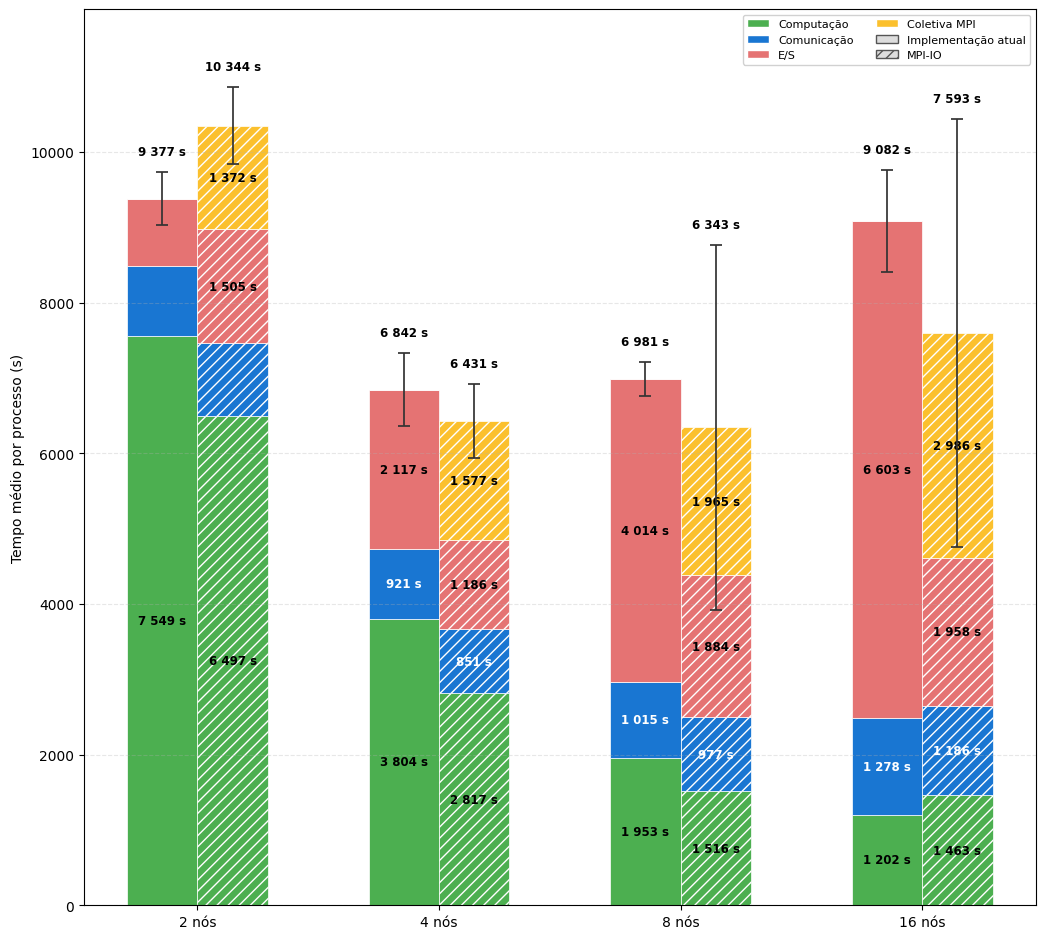
\includegraphics[width=\textwidth]{figuras/Tempo_execucao_SDumont.png}
  \caption{Decomposição do tempo médio por processo das implementações
  atual e MPI-IO no Experimento SDumont.}
  \label{fig:Tempo_execucao_SDumont}
\end{figure}

A Figura~\ref{fig:EnvioPorTamanho_SDumont} apresenta o tempo médio
de bloqueio das operações de envio em função do tamanho dos blocos
de dados no Experimento SDumont, em escala logarítmica, organizada
em quatro painéis --- um por categoria de tamanho.

O painel (a), correspondente a blocos de até 1~KB, mostra tempos de
envio na ordem de poucas dezenas de microssegundos para ambas as
implementações em todas as escalas, com diferenças marginais. Para
essa granularidade, dominada por chamadas de controle e protocolo,
nem o gargalo do escritor único nem o custo fixo da camada MPI-IO
se manifestam de forma significativa.

O painel (b), referente a blocos de até 128~KB, evidencia o
contraste mais dramático da figura. A implementação atual cresce de
$5{,}7\!\times\!10^{-5}$~s em 2~nós para $2{,}7\!\times\!10^{-3}$~s
em 8~nós e $4{,}1\!\times\!10^{-3}$~s em 32~nós, enquanto a
implementação MPI-IO permanece estável em torno de
$1{,}3\!\times\!10^{-5}$~s em todas as configurações. Nessa faixa, a
contenção do processo escritor da arquitetura atual amplifica-se
rapidamente com a concorrência, e a escrita paralela da MPI-IO chega a
apresentar vantagem de mais de duas ordens de grandeza em 32~nós.

Os painéis (c) e (d), referentes a blocos de até 1~MB e até 50~MB,
mostram um comportamento misto. Em 2 e 4~nós, a implementação atual
ainda apresenta tempos menores --- 4{,}6~ms e 21~ms na classe de
até 1~MB; 14~ms e 55~ms na classe de até 50~MB ---, enquanto a
MPI-IO paga seu custo fixo (45~ms, 71~ms, 123~ms e 250~ms,
respectivamente). Essa vantagem inicial se inverte a partir de
8~nós: a saturação do escritor único na implementação atual eleva o
tempo médio para 0{,}593~s na classe de até 1~MB e 0{,}982~s na
classe de até 50~MB, contra 0{,}094~s e 0{,}433~s da MPI-IO. Em
16~nós, a vantagem da MPI-IO consolida-se: 0{,}082~s vs.\
0{,}797~s na classe de até 1~MB (uma ordem de grandeza) e
0{,}586~s vs.\ 1{,}36~s na classe de até 50~MB. Em
32~nós, a implementação atual volta a se degradar, chegando a
2{,}90~s na classe de até 1~MB e 5{,}16~s na classe de até 50~MB,
enquanto a MPI-IO permanece em 0{,}095~s e 0{,}791~s,
respectivamente.

Em conjunto, os painéis evidenciam um ponto de troca em função da
escala: em 2 e 4~nós, a implementação atual é competitiva ou
superior em blocos médios e grandes; a partir de 8~nós, a
arquitetura MPI-IO se torna sistematicamente vantajosa em todas as
classes não triviais, com ganhos de até duas ordens de grandeza nos
blocos de até 128~KB. Esse padrão também explica diretamente o
colapso da banda agregada da implementação atual mostrado na
Figura~\ref{fig:Banda_SDumont}: a partir de 8~nós, a maior parte do
volume escrito sofre saturação no escritor único.

\begin{figure}[H]
  \centering
  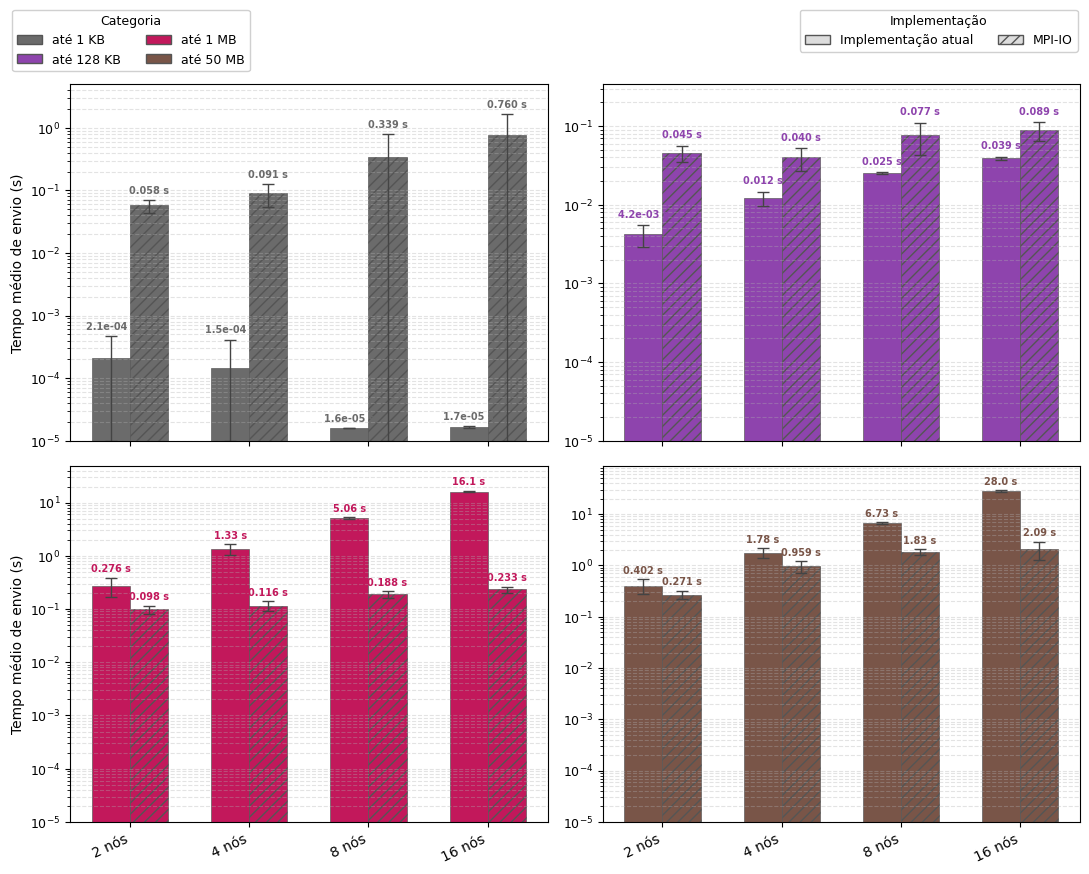
\includegraphics[width=\textwidth]{figuras/EnvioPorTamanho_SDumont.png}
  \caption{Tempo médio de bloqueio das operações de envio por tamanho de
  bloco de dados nas implementações atual e MPI-IO no Experimento SDumont
  (escala logarítmica).}
  \label{fig:EnvioPorTamanho_SDumont}
\end{figure}

Os resultados apresentados nesta seção demonstram que a adoção da
abordagem MPI-IO com escritas independentes endereça o gargalo da
arquitetura original associado à concentração das operações de E/S
no processo escritor. No SDumont, esse benefício se manifesta a
partir de 8~nós: a banda agregada cresce monotonicamente até
34{,}1~Gb/s em 32~nós, contra um perfil que colapsa e satura na
implementação atual; o tempo de E/S é reduzido em 80{,}0\%, 84{,}8\%
e 94{,}8\% em 8, 16 e 32~nós, respectivamente. Em 2 e 4~nós, o
custo fixo da camada MPI-IO ainda sobrepõe-se ao ganho de
paralelismo de escrita, e a implementação atual é ligeiramente mais
rápida. A partir de 8~nós, a MPI-IO também reduz o tempo total, com
ganho crescente até 28{,}6\% em 32~nós.

A queda de eficiência paralela observada em 32~nós --- 30{,}7\% na
implementação atual e 44{,}2\% na MPI-IO --- e a variabilidade
observada refletem, em boa medida, o caráter compartilhado do
Lustre do SDumont, em que diferentes cargas de HPC concorrem
simultaneamente pelo mesmo sistema de arquivos. Mesmo nesse cenário
hostil, o contraste qualitativo entre o perfil monotonicamente
crescente de banda da MPI-IO e o colapso da implementação atual a
partir de 8~nós persiste em toda a faixa avaliada, indicando que a
vantagem estrutural da escrita paralela se mantém quando a
infraestrutura impõe limites significativos.

% =============================================================
\section{Síntese das avaliações}
\label{sec:sintese_avaliacoes}

Os dois experimentos --- AWS, em ambiente de nuvem com FSx for Lustre
dedicado, e SDumont, em supercomputador com Lustre compartilhado
entre múltiplas cargas de HPC --- convergem para um diagnóstico
comum, ainda que com magnitudes diferentes. Em pequena escala (2 e
4~nós), a implementação atual é competitiva ou ligeiramente
superior, pois o gargalo do escritor único ainda não saturou e o
custo fixo da camada MPI-IO pesa em relação ao tempo total. A partir
de 8~nós, o quadro de E/S se inverte: a banda agregada da
implementação atual colapsa e satura, refletindo a contenção sobre
o adaptador de rede do nó escritor, enquanto a MPI-IO exibe perfil
monotonicamente crescente de banda. Esse contraste
qualitativo de comportamento --- e não apenas o ganho pontual em uma
ou outra escala --- é o resultado mais robusto deste capítulo.

A magnitude do benefício, no entanto, depende fortemente da
infraestrutura de armazenamento subjacente. No FSx for Lustre
dedicado da AWS, a abordagem proposta atinge 380{,}3~Gb/s em 32~nós
(ganho de 113$\times$ sobre a implementação atual) e reduz o tempo
total em até 36{,}7\%, com curva de banda ainda em crescimento. No
Lustre compartilhado do SDumont, a banda da MPI-IO chega a
34{,}1~Gb/s em 32~nós (ganho de 9{,}1$\times$), a redução do tempo
de E/S chega a 94{,}8\% e o tempo total cai até 28{,}6\%. Esses ganhos
ocorrem em condições adversas de concorrência por metadados e por
banda do sistema de arquivos com outras aplicações em execução. A
preservação da vantagem estrutural mesmo nesse regime sugere que a
arquitetura proposta é portátil entre ambientes heterogêneos, e não
dependente das condições idealizadas de uma plataforma dedicada.

A análise do impacto do número de OSTs na AWS reforça que o
paralelismo de armazenamento subjacente é parte essencial do ganho:
sair de 4 para 10~OSTs amplia a banda agregada em aproximadamente
5{,}6$\times$ em 16~nós e 23{,}6$\times$ em 32~nós, além de reduzir o
tempo médio das escritas nas classes de bloco maiores. Essa observação
sugere que, em deployments futuros, o dimensionamento da camada de
armazenamento --- número de OSTs e largura de \textit{stripe} ---
deve ser tratado como parâmetro de projeto, e não como detalhe
operacional.

Esses resultados não esgotam, porém, o estudo da escalabilidade da
fase de simulação final do SDDP. A faixa avaliada estendeu-se até
32~nós na AWS e no SDumont; configurações maiores podem revelar
comportamentos adicionais, em particular saturação de metadados ou
efeitos de coordenação coletiva. O custo da
Coordenação MPI-IO, que aqui se mostrou desprezível em valor
absoluto mas inflado em participação percentual pelo tamanho
reduzido das execuções de teste, merece reavaliação em cargas reais
de operação programada do SIN, com horizontes plurianuais. Por fim,
o trabalho restringiu-se à fase de simulação final, em que cenários
são mutuamente independentes; a aplicabilidade da estratégia à fase
de convergência, com seu padrão diferente de comunicação e
sincronização, fica como tema natural de continuidade.


%===============================================================================
\chapter{Trabalhos relacionados}
\label{cap:trabalhos_relacionados}

O trabalho de \citeauthor{Dickens:08}~\cite{Dickens:08} introduziu o uso de MPI-IO
sobre o Lustre, identificando que as premissas de otimização do ROMIO conflitam com
o modelo de byte-range locking do filesystem: para padrões não-interleaved, nos quais
cada processo escreve em uma região exclusiva, escritas independentes evitam contenção
de locks e superam as coletivas em desempenho.
Esse diagnóstico abriu uma linha de pesquisa diretamente relevante para este trabalho,
explorada em~\cite{Dickens:10}, \cite{LiaoIPDPS:07}, \cite{Gropp:08} e~\cite{Liao:08},
e fundamenta a escolha de \texttt{MPI\_File\_write\_at} como primitiva de E/S paralela
no SDDP.

\citeauthor{LiaoIPDPS:07}~\cite{LiaoIPDPS:07} demonstraram que escritas
independentes cujo tamanho não preenche uma unidade de \textit{stripe} do
Lustre forçam a aquisição de múltiplos locks sequenciais, degradando o
desempenho. Como solução, os autores propuseram um mecanismo de
\textit{two-stage write-behind buffering} que acumula dados em memória até
completar um bloco alinhado à fronteira de \textit{stripe} antes de emitir a
escrita ao filesystem. Esta dissertação \emph{não adotou} essa abordagem: a implementação descrita no Capítulo~\ref{cap:proposta}
apenas agrega os registros horários por par
$(\text{estágio}, \text{cenário})$ em uma única escrita, sem
alinhamento explícito às fronteiras de \textit{stripe}. Ainda assim,
parte das escritas resultantes \emph{acaba se alinhando
incidentalmente} ao tamanho de \textit{stripe} configurado no Lustre
(1~MB nos experimentos), em decorrência do padrão de acesso do SDDP
no formato horário: arquivos com algumas centenas de elementos do
sistema elétrico produzem blocos por par
$(\text{estágio}, \text{cenário})$ próximos ou múltiplos da fronteira
de \textit{stripe} (cf.~Seção~\ref{sec:formato_resultados}). Esse
alinhamento incidental tende a beneficiar parte das operações de E/S
do SDDP --- evitando, para esses blocos, a aquisição de múltiplos
locks descrita por \citeauthor{LiaoIPDPS:07} --- e ajuda a explicar o
desempenho já obtido pela arquitetura proposta mesmo na ausência de
um mecanismo explícito de bufferização alinhada. A incorporação
\emph{sistemática} desse alinhamento permanece como direção de
aprimoramento da arquitetura proposta, beneficiando inclusive os arquivos
cujos blocos por cenário ficam desalinhados.

Em continuação direta, \citeauthor{Dickens:10}~\cite{Dickens:10} propuseram a Y-lib,
uma biblioteca que substitui o driver ADIO padrão do ROMIO para Lustre, implementando
hierarchical striping e split writing para alinhar as operações de E/S às fronteiras
de stripe e reduzir a contenção de locks. Os experimentos reportados pelos autores
mostram ganhos de até 220\% sobre a implementação padrão, confirmando que o Lustre
requer tratamento específico para extrair desempenho em escritas paralelas.

\citeauthor{Gropp:08}~\cite{Gropp:08} formalizaram que, quando os acessos de
diferentes processos não são interleaved --- isto é, cada processo escreve em
uma região exclusiva do arquivo ---, a chamada \texttt{MPI\_File\_write\_all}
degenera para \texttt{MPI\_File\_write} acrescida de overhead de sincronização,
tornando as escritas coletivas estritamente piores do que as independentes nesse
regime. Esse resultado fundamenta teoricamente a escolha de
\texttt{MPI\_File\_write\_at} no SDDP, cujo padrão de acesso é precisamente
não-interleaved.

\citeauthor{Liao:08}~\cite{Liao:08} mostraram que o particionamento de
\textit{file domains} do two-phase I/O do ROMIO não coincide com as fronteiras
de \textit{stripe} do Lustre, gerando contenção de locks mesmo em operações
coletivas bem-formadas. Os autores propuseram um particionamento adaptativo
ao protocolo de locking do filesystem subjacente, reduzindo essa contenção.
Esse resultado complementa \cite{Dickens:08}, reforçando que, para o padrão
de acesso do SDDP, escritas independentes com offsets pré-calculados evitam
inteiramente o problema de particionamento identificado pelos autores.

\citeauthor{GarciaCarballeiraISPDC:23}~\cite{GarciaCarballeiraISPDC:23}
apresentam o \emph{Expand Ad-Hoc}, um sistema de arquivos paralelo
\textit{ad-hoc} baseado em servidores MPI em espaço de usuário que
virtualiza o armazenamento local dos nós de computação --- SSDs ou
memória compartilhada --- em um volume efêmero, cujo ciclo de vida
coincide com o do \textit{job} submetido: a aplicação escreve nesse
volume durante a execução e a sincronização com o \textit{backend}
persistente (Lustre, GPFS) ocorre apenas nas etapas de
\textit{stage-in} e \textit{stage-out}, fora da janela crítica da
computação. Essa abordagem é diretamente relevante para a
degradação observada no Experimento SDumont
(Subseções~\ref{sec:sdumont_atual} e~\ref{sec:sdumont_mpiio}), em
que a concorrência entre o \textit{job} do SDDP e outras cargas de
HPC sobre o mesmo Lustre compartilhado impôs um teto absoluto de
banda (34{,}1~Gb/s em 32~nós) uma ordem de grandeza inferior ao
obtido na AWS com FSx for Lustre dedicado (380{,}3~Gb/s). Compor o
MPI-IO com escritas independentes sobre uma camada como o Expand
Ad-Hoc, instanciada nos próprios nós alocados ao \textit{job} SDDP,
contornaria inteiramente essa contenção externa, com migração ao
Lustre apenas no \textit{stage-out} final, e tem potencial de
aproximar o desempenho observado no SDumont do desempenho obtido em
um \textit{backend} dedicado.

%===============================================================================
\chapter{Conclusões e trabalhos futuros}
\label{cap:conclusao}

Esta dissertação investigou os gargalos de E/S da fase de simulação
final do algoritmo SDDP e propôs uma arquitetura paralela baseada em
escritas independentes com MPI-IO sobre o sistema de arquivos
Lustre, substituindo a estratégia atual com processo escritor único.
A avaliação experimental conduzida em dois ambientes distintos ---
AWS (FSx for Lustre dedicado) e Santos Dumont (LNCC, Lustre
compartilhado) --- confirma que a arquitetura proposta endereça
efetivamente o gargalo identificado e produz ganhos expressivos de
desempenho e escalabilidade.

Na configuração de 32 nós, a arquitetura MPI-IO reduz o tempo total
de execução em 36{,}7\% no Experimento AWS e em 40{,}4\% no Experimento
SDumont, em relação à implementação atual. A banda agregada
percebida pela aplicação cresce em 113$\times$ na AWS e
13,7$\times$ no SDumont. O contraste qualitativo entre as duas
implementações é tão relevante quanto a magnitude desses ganhos:
enquanto a implementação atual exibe colapso da banda a partir de
8~nós na AWS e de 16~nós no SDumont --- decorrente da serialização
inerente à implementação centralizada em um único processo escritor ---, a implementação proposta apresenta perfil
monotonicamente crescente de banda em toda a faixa avaliada,
indicando que a infraestrutura de armazenamento ainda não atingiu
seu limite nominal. Esse comportamento se sustenta em ambos os
ambientes, atestando a portabilidade da solução entre
infraestruturas heterogêneas --- nuvem dedicada e supercomputador
compartilhado.

A análise do impacto do número de \textit{Object Storage Targets}
(OSTs) reforça que o dimensionamento da camada de armazenamento é
parte essencial do ganho: passar de 4 para 10~OSTs no FSx for
Lustre amplia a banda agregada percebida em aproximadamente
5,6$\times$ em 16~nós e 23,6$\times$ em 32~nós, com redução do
tempo médio das escritas nas classes de bloco maiores. Esse
resultado sugere que, em \textit{deployments} futuros, o
\texttt{stripe\_count} e o \texttt{stripe\_size} do Lustre devem
constituir parâmetros de projeto, e não um detalhe
operacional.

\paragraph{Padrão de acesso dos arquivos diários.} Dos 117 arquivos
de resultado produzidos pelo SDDP nos experimentos, 104 seguem o
formato horário e 13 seguem o formato diário. Embora minoritários
em quantidade, os arquivos diários respondem por todas as escritas
de blocos muito pequenos observadas no \textit{workload}: cada
registro corresponde a um dia do mês e, diferentemente dos arquivos
horários --- nos quais a aplicação agrega os registros horários de um par
$(\text{estágio}, \text{cenário})$ em uma única escrita ---, ela não agrupa
os dias nos arquivos diários. A
sobreposição entre E/S e computação proporcionada pelas escritas
assíncronas mitiga parcialmente o impacto desse padrão fragmentado, mas a
frequência de pequenas requisições ao Lustre permanece como fonte residual
de sobrecarga e direciona uma das linhas de continuidade deste trabalho.

\paragraph{Disponibilidade de instâncias na nuvem.} A execução do
Experimento AWS enfrentou dificuldades de disponibilidade de
instâncias \texttt{r7i.12xlarge} na mesma região, dado o caráter
\textit{memory-optimized} dessa família e a demanda concorrente
sobre o \textit{pool} de recursos. Essa limitação operacional
restringiu a janela de experimentação, e o planejamento de futuras
execuções em nuvem para cargas HPC deve considerá-la.

\section*{Trabalhos futuros}

A partir dos resultados e limitações apresentados, este trabalho
identifica as seguintes direções de continuidade:

\begin{itemize}
  \item \textbf{Reorganização do padrão de acesso dos arquivos
        diários}, agrupando os registros mensais em uma única
        escrita por $(\text{estágio}, \text{cenário})$ ---
        analogamente ao que a aplicação já faz nos arquivos horários ---,
        de modo a eliminar a parcela residual de pequenas
        requisições ao Lustre identificada nestes experimentos.

  \item \textbf{Avaliação com adaptadores de rede de alta
        velocidade}, como InfiniBand HDR/NDR e \textit{Elastic
        Fabric Adapter} (EFA) da AWS, para investigar em que
        medida a rede deixa de ser fator limitante e como o custo
        da Coordenação MPI-IO escala em redes de baixa latência.

  \item \textbf{Sensibilidade ao tamanho de \textit{stripe} do
        Lustre}, com experimentos variando o \texttt{stripe\_size}
        para mapear o \textit{trade-off} entre fragmentação das
        requisições e distribuição efetiva entre os OSTs.

  \item \textbf{Buferização alinhada às \textit{stripes} do Lustre},
        substituindo o esquema atual --- em que cada \textit{rank}
        acumula em memória o bloco correspondente ao estágio
        completo de um cenário antes de submetê-lo em uma única
        chamada \texttt{MPI\_File\_iwrite\_at} ou
        \texttt{MPI\_File\_write\_at} --- por uma política que
        segmente as escritas pelos limites das \textit{stripes}, de
        modo que cada submissão MPI-IO incida sobre exatamente uma
        \textit{stripe} e, portanto, sobre exatamente um OST.
        Liao~\textit{et al.}~\cite{LiaoIPDPS:07} demonstram, em um
        contexto mais geral de escritas independentes em MPI-IO,
        que um esquema de bufferização em dois estágios alinhado ao
        particionamento do sistema de arquivos paralelo melhora
        significativamente o desempenho das escritas pequenas e
        desalinhadas; o mesmo princípio aplica-se diretamente ao
        perfil de E/S do SDDP horário, com potencial de reduzir a
        contenção entre \textit{ranks} concorrentes sobre os mesmos
        OSTs.

  \item \textbf{Sensibilidade ao limite síncrono/assíncrono}, com
        experimentos variando o ponto de corte entre escritas
        assíncronas e síncronas (por exemplo, 64, 128 e
        256~KB) para refinar empiricamente o parâmetro de projeto
        adotado neste trabalho.

  \item \textbf{Avaliação de \textit{two-phase I/O}}, isto é, de
        escritas coletivas com agregação interna pela biblioteca
        MPI-IO. Tentativas preliminares conduzidas durante esta
        pesquisa resultaram em \textit{deadlock}, atribuído à
        combinação de múltiplas escritas por cenário com o
        desalinhamento do número de cenários processados por cada
        \textit{rank} no padrão \textit{bag-of-tasks}. A
        viabilização dessa estratégia exigiria mecanismos de
        sincronização que reconciliem a natureza dinâmica da
        distribuição de tarefas com a semântica coletiva das
        operações de E/S.

  \item \textbf{Diagnóstico das variações no tempo de computação para
        uma mesma configuração}, caracterizando as flutuações
        observadas na fase de computação entre execuções com o mesmo
        número de nós. Como discutido na Seção~\ref{sec:sintese_avaliacoes},
        a eficiência paralela permanece abaixo do ideal linear no
        regime de \textit{strong scaling}: com o problema de tamanho
        fixo, custos aproximadamente constantes da computação ---
        sobretudo os associados ao acesso à memória --- deixam de ser
        amortizados à medida que se adicionam nós. A investigação
        detalhada desse gargalo computacional, distinto do gargalo de
        E/S tratado nesta dissertação (por exemplo, via
        \textit{profiling} da hierarquia de memória e da largura de
        banda de acesso), permitiria isolar seus efeitos dos de E/S e
        orientar otimizações futuras da fase de simulação.

  \item \textbf{Investigação da piora pontual observada em 4~nós no
        Experimento AWS} (Seção~\ref{sec:avaliacao_comparativa_aws}),
        em que o tempo total da implementação MPI-IO superou o da
        implementação atual apesar do ganho já mensurável de banda.
        Esse resultado é indício de que fatores externos ao módulo de
        E/S --- possivelmente variações no tempo de computação entre
        repetições --- dominaram esse ponto específico da curva. Sua
        caracterização, articulada com o diagnóstico das variações de
        computação mencionado acima, ajudaria a separar os efeitos de
        E/S dos efeitos computacionais na análise de escalabilidade.

  \item \textbf{Extensão da arquitetura à fase de geração de cortes do
        SDDP}, avaliando em que medida a estratégia de escritas
        independentes com MPI-IO se aplica ao padrão de comunicação e
        de sincronização dessa fase, distinto do da fase de simulação
        final tratada nesta dissertação.
\end{itemize}

A consolidação dessas direções pode contribuir para a construção de
uma arquitetura de E/S ainda mais escalável e portátil, aplicável
não apenas ao SDDP, mas a uma classe mais ampla de aplicações
científicas com padrões \textit{bag-of-tasks} e produção intensiva
de resultados.


  \backmatter

  \bibliographystyle{coppe-unsrt}
  \bibliography{bibliografy}

\end{document}
